\documentclass[a4paper,11pt]{article}
\usepackage{cmap}
\usepackage[T1]{fontenc}
\usepackage[utf8]{inputenc}
\usepackage{lmodern}
\usepackage{microtype}
\usepackage{textcomp}
\usepackage[spanish,es-tabla]{babel}
\usepackage[a4paper,left=2.5cm,right=2.5cm,top=2.4cm,bottom=2.4cm]{geometry}
\usepackage{graphicx}
\usepackage{booktabs}
\usepackage{array}
\usepackage{amsmath,amssymb}
\usepackage{hyperref}
\usepackage{enumitem}
\usepackage{xcolor}
\usepackage{eurosym}

\hypersetup{
    colorlinks=true,
    linkcolor=black,
    citecolor=black,
    urlcolor=blue!70!black
}
\setlength{\parskip}{0.8ex}
\setlength{\parindent}{0pt}

\begin{document}

\begin{center}
\vspace*{1mm}
{\Large \textbf{Centro de Cómputo Low-Cost: Estudio Experimental de Viabilidad}}\\[2mm]
{\normalsize Reutilización e Integración de GPUs Heterogéneas y \textit{Legacy} en Plataformas Modernas}\\[4mm]
{\small \textbf{Marina Delgado Trinidade}}\\[1mm]
\end{center}
\vspace{2mm}
\hrule
\vspace{3mm}

\section{Introducción y Pregunta de Investigación}

Este proyecto se centra en el estudio experimental de la viabilidad de aprovechar múltiples GPUs
—pudiendo ser distintas generaciones, arquitecturas y fabricantes— dentro de un mismo sistema,
siendo lo óptimo poder utilizar todas ellas sin necesidad de descartar ninguna. El objetivo general es
determinar hasta qué punto es posible integrar tarjetas de dicha índole e implementarlas en una máquina de
cómputo obteniendo un rendimiento conjunto útil, empleando hardware de segunda mano o legacy.

La pregunta central que guía este Trabajo de Fin de Grado es: \textbf{¿Bajo qué condiciones técnicas y operativas es viable reutilizar GPUs heterogéneas y \textit{legacy} en un sistema de consumo moderno para obtener un rendimiento de cómputo útil?}

El trabajo no persigue encontrar una solución óptima para una versión de kernel o unas especificaciones concretas, sino \textbf{determinar bajo qué condiciones la integración es viable y bajo cuáles deja de compensar}, a partir de un caso de estudio real construido y medido.

\section{Arquitectura del Sistema Experimental}

\begin{center}
\small
\begin{tabular}{lp{10.2cm}}
\toprule
\textbf{Componente} & \textbf{Especificación / Rol en el sistema} \\
\midrule
\textbf{Placa Base} & ASUS TUF GAMING X670E-PLUS WIFI (Plataforma AM5 de consumo) \\
\textbf{Procesador (CPU)} & AMD Ryzen 9 7950X (16 núcleos / 32 hilos, 28 líneas PCIe 5.0) \\
\textbf{Hipervisor Anfitrión} & Proxmox VE 9.2 (Basado en Debian 12, \textit{Kernel} Linux 6.14) \\
\textbf{GPU 1 (Cómputo)} & NVIDIA Tesla C1060 (Arquitectura GT200GL, 240 cores CUDA, 4 GB VRAM) \\
\textbf{GPU 2 (Cómputo)} & NVIDIA Tesla C1060 (Arquitectura GT200GL, 240 cores CUDA, 4 GB VRAM) \\
\textbf{GPU 3 (Cómputo)} & ASUS GeForce GTS 250 (Arquitectura G92b, 128 cores CUDA, 1 GB VRAM) \\
\textbf{Controlador Base} & NVIDIA 340.108 (Última versión compatible con Compute Capability $<$ 2.0) \\
\textbf{Plataforma de Cómputo} & CUDA Toolkit 6.5 (Última versión con soporte para arquitecturas \texttt{sm\_11} y \texttt{sm\_13}) \\
\textbf{Configuración PCIe} & Enlace forzado a PCIe 1.0 (Gen1) desde la BIOS para garantizar los tiempos de negociación del enlace \\
\bottomrule
\end{tabular}
\end{center}

Todas las tarjetas comparten la misma generación de controlador propietario (rama 340.xx), permitiendo validar tanto
estrategias de virtualización completa como de aislamiento ligero.

\section{Fundamentos Teóricos Aplicados}

En esta sección se propone un marco teórico que permita decidir a priori si un sistema de reaprovechamiento con GPUs de consumo es
viable.
El modelo consta de cinco filtros con valor en $[0,1]$, donde $1$ indica un resultado favorable y $0$ la inviabilidad. Se combinan
mediante un producto que conserva la semántica conjuntiva pero admite filtros graduados, penalizando proporcionalmente cualquier
degradación sin exigir un todo o nada:
\begin{equation*}
V = \prod_{i} F_i = F_{\text{driver}} \cdot F_{\text{aislamiento}} \cdot F_{\text{carga}} \cdot F_{\text{coste}} \cdot F_{\text{estabilidad}}
\end{equation*}
\begin{itemize}[leftmargin=*,labelsep=0.5em,itemsep=0.8ex]
    \item \textbf{$F_{\text{driver}}$ (Compatibilidad del software base):} Se estudia si el código del controlador propietario puede compilarse y enlazarse en \textit{kernels} contemporáneos (mediante
    DKMS u otro gestor de módulos de kernel y parches de compatibilidad) sin comprometer la estabilidad del sistema
    anfitrión. 
    \item \textbf{$F_{\text{aislamiento}}$ (Virtualización y orquestación):} Si las GPUs requieren versiones de drivers
    incompatibles entre sí, no pueden convivir en el mismo \textit{kernel} anfitrión y deben aislarse en máquinas
    virtuales mediante VFIO \textit{passthrough}, lo que exige una segmentación IOMMU limpia y soporte de reinicio (FLR).
    Parámetro opcional relativo a cuando se cumple este escenario. En caso contrario, 
    no es necesario el aislamiento mediante VFIO y este parámetro no aplica, por lo que se considera favorable ($F_{\text{aislamiento}} = 1$).
    \item \textbf{$F_{\text{carga}}$ (Intensidad de la carga de trabajo):} Determina si el cuello de botella reside en las
    limitaciones de las comunicaciones del bus PCIe (negociaciones, sincronización, velocidad de transferencia...) o si, por otro
    lado, la limitación reside en el tiempo de procesado de cálculo. Problema de tipo Transfer Bound frente a Compute Bound.
    Se formaliza de forma graduada a partir del modelo Roofline en la sección~\ref{sec:roofline}.
    \item \textbf{$F_{\text{coste}}$ (Viabilidad económica y operativa):} Comprueba si el valor del cómputo obtenido supera el coste
    energético, las horas de ingeniería invertidas y el riesgo de obsolescencia.
    \item \textbf{$F_{\text{estabilidad}}$ (Resiliencia operativa):} Mide la tasa de fallos, bloqueos del bus o eventos críticos
    durante ejecuciones sostenidas en el tiempo. Dado que los fallos de hardware no son deterministas, pueden haberse superado con éxito
    los cuatro parámetros anteriores y aún así encontrarnos con situaciones limitantes en la parte experimental.
\end{itemize}

% ---------------------------------------------------------------------------
\subsection{Leyes de Escalado (Amdahl y Gustafson)}

Se eligen estas leyes ya que nos permiten analizar el escalado en el rendimiento de un sistema a medida que aumentan los recursos, que
en nuestro caso concreto, se traduce en ir añadiendo GPUs.

\subsubsection*{Ley de Amdahl}

La ley de Amdahl es la siguiente:
\begin{equation}\label{eq:amdahl}
    T_{\text{mejorado}} = T_{\text{antes}} \left( (1 - f_{\text{m}}) + \frac{f_{\text{m}}}{A_{\text{m}}} \right)
\end{equation}
\begin{itemize}[leftmargin=*,noitemsep,topsep=2pt]
    \item $T_{\text{antes}}$: Tiempo total de ejecución base previo al aumento de recursos.
    \item $f_{\text{m}}$: Fracción del tiempo de cómputo original que se ve directamente beneficiada por la mejora ($0 \le f_{\text{m}} \le 1$).
    \item $1 - f_{\text{m}}$: Fracción inalterada por ser estrictamente secuencial, y que por tanto,
    no experimenta aceleración alguna.
    \item $A_{\text{m}}$: Factor de aceleración local (\textit{speedup}) obtenido exclusivamente en la parte 
    mejorada (adimensional; en paralelismo ideal con $n$ GPUs homogéneas, $A_{\text{m}} = n$).
\end{itemize}

En arquitectura de computadores, la aceleración de un sistema por definición es:
\begin{equation}\label{eq:speedup}
    S(n) = \frac{T_{\text{antes}}}{T_{\text{mejorado}}}
\end{equation}
Por lo que si sustituimos la expresión de tiempo mejorado de \eqref{eq:amdahl} en \eqref{eq:speedup}:
\begin{equation}
    S(n) = \frac{T_{\text{antes}}}{T_{\text{mejorado}}}
         = \frac{T_{\text{antes}}}{T_{\text{antes}} \left( (1 - f_{\text{m}}) + \dfrac{f_{\text{m}}}{A_{\text{m}}} \right)}
\end{equation}
Simplificando se nos queda en:
\begin{equation}\label{eq:amdahl_speedup}
    S(n) = \frac{1}{(1 - f_{\text{m}}) + \dfrac{f_{\text{m}}}{A_{\text{m}}}}
\end{equation}

La Ley de Amdahl permite modelar la aceleración teórica máxima ($S$) al paralelizar una carga de trabajo sobre $n$ recursos~\cite{amdahl1967}. Sin
embargo, impone una limitación asintótica insalvable: incluso en el caso ideal en el que el número de recursos tienda a
infinito ($n \to \infty$, tomando $A_{\text{m}} = n$), la aceleración queda estrictamente acotada por la fracción no paralelizable:
\begin{equation}\label{eq:amdahl_limite}
    \lim_{n \to \infty} S(n) = \frac{1}{1 - f_{\text{m}}}
\end{equation}
En el contexto de este trabajo, dicho término secuencial ($1 - f_{\text{m}}$) no comprende únicamente las secciones de código
no paralelizables, sino que abarca también los tiempos de sincronización y las latencias físicas de transferencia
de datos del bus PCIe. Esta sobrecarga puede situar al sistema en un régimen limitado por transferencia (\textit{transfer-bound}),
donde el bus actúa como el cuello de botella crítico frente a la capacidad de cálculo pura de las GPUs.

Para mitigar esta limitación de tanto peso, la estrategia consiste en reducir el tráfico que atraviesa el bus elevando la
intensidad aritmética de la implementación: reutilizar cada byte transferido en el mayor número posible de operaciones
(bloqueo o \textit{tiling}, residencia de los datos en VRAM, solapamiento de transferencia y cálculo mediante \textit{streams}).
Conviene subrayar que esta adaptación no siempre es posible: una implementación concreta de un algoritmo posee un techo de
intensidad alcanzable $I_{\text{A}}^{\max}$, impuesto por su estructura y por la capacidad de reutilización de memoria
disponible. La compensación de la asimetría del bus solo es viable mientras ese techo supere el punto de cresta del sistema:
\begin{equation}\label{eq:i_max}
    I_{\text{A}}^{\max} \ge I_{\text{A}}^* = \frac{P_{\text{pico}}}{AB}
\end{equation}
Si, por el contrario, $I_{\text{A}}^{\max} < I_{\text{A}}^*$, el problema es intrínsecamente \textit{transfer-bound} para esa
GPU y esa ranura: ninguna optimización de software elimina la cota y la única vía de viabilidad pasa por aumentar el ancho de
banda del enlace. Es más, la frontera no es una propiedad absoluta del algoritmo, sino del par algoritmo--hardware: una misma
carga puede ser \textit{compute-bound} en una máquina moderna y \textit{transfer-bound} en esta plataforma, con enlaces Gen1
y una ranura x4 compartida a través del \textit{chipset}.

En sistemas heterogéneos, sin embargo, la igualdad $A_{\text{m}} = n$ deja de cumplirse, ya que no todas las GPUs aportan
la misma capacidad de cálculo. Tomando como referencia el rendimiento de la GPU más rápida ($P_{\text{ref}}$) y suponiendo un
reparto de la carga proporcional a la capacidad de cada tarjeta, el factor de aceleración local es:
\begin{equation}\label{eq:am_proporcional}
    A_{\text{m}} = \frac{\sum_{i=1}^{n} P_i}{P_{\text{ref}}}
\end{equation}
donde $P_i$ es el rendimiento individual de cada GPU. Con los valores medidos en la Fase 4 (Tesla C1060: 155.26 GFlop/s;
GTS 250: 80.49 GFlop/s), la combinación de ambas tarjetas proporciona $A_{\text{m}} \approx 1.52$ en lugar de 2. Suponiendo
que la segunda Tesla C1060 rinde igual que la primera, el sistema completo con las tres GPUs alcanzaría
$A_{\text{m}} \approx 2.52$ en lugar de 3.

Si, por el contrario, la carga se reparte a partes iguales entre las GPUs, la más lenta ($P_{\min}$) determina el tiempo total:
\begin{equation}\label{eq:am_equitativo}
    A_{\text{m}} = n \cdot \frac{P_{\min}}{P_{\text{ref}}}
\end{equation}
lo que en el caso de la Tesla C1060 junto a la GTS 250 resulta en $A_{\text{m}} \approx 1.04$: la segunda tarjeta apenas aporta
aceleración. Por tanto, en sistemas heterogéneos el criterio de reparto de la carga resulta tan determinante como el número de
GPUs que se añaden.

\subsubsection*{Ley de Gustafson}

La Ley de Gustafson matiza la cota impuesta por Amdahl, según la cual el factor de aceleración siempre queda limitado por la fracción
secuencial sin importar con cuántos recursos se mejore un sistema. Más específicamente, la formulación de Gustafson complementa la perspectiva
de Amdahl adaptando el modelo al escalado débil (\textit{weak scaling}), donde el tamaño del problema crece proporcionalmente con la capacidad
en recursos del sistema, manteniendo constante el tiempo de
ejecución ($T_{\text{mejorado}}$).
En otras palabras, se pone énfasis en que en un sistema con mayores recursos, pueden abordarse problemas de mayor complejidad
computacional. En el caso de estudio que nos concierne, la compensación se obtiene en la medida en que el tiempo dedicado al cálculo crece más
deprisa que el invertido en transferencias, justo la situación que se busca para paliar la asimetría del bus PCIe~\cite{gustafson1988}.

A diferencia de la formulación de Amdahl, donde la fracción de tiempo mejorada $f_{\text{m}}$ se define sobre el tiempo del sistema base
($T_{\text{antes}}$), en la Ley de Gustafson la fracción susceptible de mejora ($f_{\text{m}}'$) se mide directamente en el
sistema paralelo:
\begin{equation}\label{eq:gustafson_relacionada}
\begin{split}
    S = \frac{T_{\text{antes}}}{T_{\text{mejorado}}}
      &= (1 - f_{\text{m}}') + A_{\text{m}} \cdot f_{\text{m}}' \\
      &= 1 + (A_{\text{m}} - 1) \cdot f_{\text{m}}'
\end{split}
\end{equation}
donde:
\begin{itemize}[leftmargin=*,noitemsep,topsep=2pt]
    \item $S$ es la aceleración escalada del sistema completo. Dado que en el escalado débil $T_{\text{mejorado}}$ se
    mantiene constante, $T_{\text{antes}}$ no es un tiempo medido, sino el tiempo que tardaría el sistema base en
    resolver el problema ya escalado.
    \item $f_{\text{m}}'$ es la fracción del tiempo de cómputo dedicada a la fase paralela en el sistema mejorado ($0 \le f_{\text{m}}' \le 1$).
    \item $1 - f_{\text{m}}'$ representa la fracción de tiempo consumida por el código secuencial, las sincronizaciones y las transferencias por el bus.
    \item $A_{\text{m}}$ es la capacidad de paralelización del entorno (en sistemas homogéneos de $n$ unidades de cálculo, $A_{\text{m}} = n$).
\end{itemize}

Esta ley evidencia que, al aumentar la dimensión de los datos a procesar, el término $A_{\text{m}} \cdot f_{\text{m}}'$ domina
frente a las sobrecargas del bus ($1 - f_{\text{m}}'$), permitiendo un crecimiento prácticamente lineal de la aceleración con respecto al
número de recursos y amortizando la latencia del enlace PCIe. Esta amortización, no obstante, exige que la intensidad aritmética
del algoritmo crezca con el tamaño del problema (como ocurre en el producto denso de matrices, con $O(N^3)$ FLOPs frente a
$O(N^2)$ bytes): en algoritmos de intensidad constante o decreciente con la escala, agrandar el problema no reduce la fracción
de tiempo dedicada al bus, y la Ley de Gustafson no ofrece ninguna escapatoria.
Esta conclusión respalda la hipótesis de trabajo: un sistema de estas características puede resultar viable 
para problemas de índole Compute Bound cuya intensidad alcanzable supere el punto de cresta, pero no para el caso de Transfer Bound.

% ---------------------------------------------------------------------------
\subsection{Modelo Roofline}\label{sec:roofline}

El modelo Roofline~\cite{williams2009} delimita el rendimiento máximo teórico que puede alcanzar una GPU ante una carga de trabajo concreta.
Caracteriza cada algoritmo en función de su \textit{Intensidad Aritmética}, la cual se define como:
\begin{equation}\label{eq:intensidad}
    I_{\text{A}} = \frac{\text{FLOPs}}{\text{Bytes transferidos}} \quad \left[\text{FLOP/Byte}\right]
\end{equation}
En su formulación clásica, los bytes transferidos son los que se mueven entre la memoria de la GPU (VRAM) y sus núcleos.
En este trabajo el modelo se adapta tomando como referencia los bytes que atraviesan el bus PCIe, ya que es el canal por el
que llegan los datos desde el anfitrión y el principal cuello de botella de la plataforma.
Ambos techos coexisten: el de la VRAM limita la ejecución del \textit{kernel} una vez los datos residen en la GPU, mientras
que el del bus PCIe limita el trabajo completo (transferencia de entrada, cálculo y devolución de resultados), que es el
que interesa en un sistema con varias GPUs que comparten el bus. Las medidas de \texttt{matrixMul} de la Fase 4
corresponden al primer caso, ya que solo cronometran la ejecución del \textit{kernel}.

El valor de esta variable marca la frontera entre los dos tipos de problemas: \textit{Transfer-Bound} y \textit{Compute-Bound}.

\begin{itemize}[leftmargin=*,noitemsep,topsep=2pt]
    \item ¿$I_{\text{A}}$ alta? Problema de naturaleza \textit{Compute-Bound}. FLOPs $\gg$ Bytes, ergo el tiempo de
    intervención del bus es despreciable frente al tiempo de cálculo.
    \item ¿$I_{\text{A}}$ baja? Problema de naturaleza \textit{Transfer-Bound}. Bytes $\gg$ FLOPs, predomina la
    comunicación frente al tiempo de cómputo, por lo que el ancho de banda del bus se convierte en el factor crítico
    de rendimiento.
\end{itemize}

Basándonos en este modelo, el rendimiento alcanzable se define como:
\begin{equation}\label{eq:roofline}
    P = \min\left(P_{\text{pico}},\; I_{\text{A}} \times AB\right) \quad \left[\text{FLOP/s}\right]
\end{equation}
donde:
\begin{itemize}[leftmargin=*,noitemsep,topsep=2pt]
    \item $P_{\text{pico}}$ (FLOP/s): Techo de cómputo. Potencia de cálculo sostenible de la GPU, tomada del mejor
    \textit{kernel} de referencia medido en la Fase 4 (155.26 GFlop/s en la Tesla C1060 y 80.49 GFlop/s en la GTS 250).
    \item $AB$ (Bytes/s): Ancho de banda efectivo del bus PCIe. Se toman los valores medidos con \texttt{bandwidthTest}
    en la Fase 4 ($\approx 1.6$ GB/s en la Tesla C1060 y $\approx 0.78$ GB/s en la GTS 250), de modo que cada GPU
    tiene su propio techo de transferencia en función de la ranura que ocupa.
    \item $I_{\text{A}} \times AB$ (FLOP/s): Techo de transferencia. Marca la tasa máxima de operaciones que la tarjeta
    puede procesar atendiendo a la velocidad con la que le llegan los datos.
\end{itemize}

El cociente entre el rendimiento alcanzable y el pico de cómputo define el filtro de carga de forma graduada:
\begin{equation}\label{eq:f_carga}
    F_{\text{carga}} = \frac{P}{P_{\text{pico}}}
                    = \min\left(1,\; \frac{I_{\text{A}} \cdot AB}{P_{\text{pico}}}\right)
                    = \min(1, \alpha), \qquad
    \alpha = \frac{I_{\text{A}}}{I_{\text{A}}^*}, \quad I_{\text{A}}^* = \frac{P_{\text{pico}}}{AB}
\end{equation}
donde $I_{\text{A}}^*$ es la intensidad aritmética del punto de cresta (\textit{ridge point}). $F_{\text{carga}}$ mide la fracción
del pico de cómputo que la carga es capaz de cosechar dada la cota del bus: vale $1$ en cuanto $I_{\text{A}} \ge I_{\text{A}}^*$
(régimen \textit{compute-bound}) y decae de forma continua conforme $I_{\text{A}}$ se aleja del punto de cresta, sin transición
abrupta. La optimización solo puede elevar $I_{\text{A}}$ hasta el techo algorítmico $I_{\text{A}}^{\max}$ (ecuación~\eqref{eq:i_max}),
de modo que $F_{\text{carga}}$ queda acotado por $\min(1,\, I_{\text{A}}^{\max} \cdot AB / P_{\text{pico}})$: si esa cota es muy
inferior a $1$, el problema resulta inviable en esta plataforma por mucho que se adapte el software. Esta definición gradual resulta más honesta que un umbral duro, ya que $P_{\text{pico}}$ y $AB$ son magnitudes medidas
con incertidumbre asociada. Si se desea un veredicto binario, el umbral se fija una única vez sobre el valor compuesto
($V \ge \tau_V$) y se justifica explícitamente en la metodología.

De entre ambos techos, se toma como indicador de rendimiento del sistema el mínimo, ya que el rendimiento queda
siempre limitado por la medida más restrictiva. Cabe destacar que esta cota supone un solapamiento perfecto entre
transferencia y cálculo, es decir, que la GPU procesa unos datos mientras recibe los siguientes (copias asíncronas
mediante \textit{streams}). Si las transferencias y el cálculo se ejecutan de forma secuencial, los tiempos se suman,
caso que recoge el modelo de la sección~\ref{sec:topologia}. Ambos modelos son, por tanto, complementarios: el Roofline
proporciona la cota superior con solapamiento y el modelo de contención, el tiempo sin él.


% ---------------------------------------------------------------------------
\subsection{Topología PCIe y Modelo de Contención}\label{sec:topologia}

En la plataforma de consumo objeto de análisis, la ranura principal tiene conexión dedicada con la CPU,
mientras que la secundaria opera eléctricamente a cuatro carriles (x4) a través del \textit{chipset}, compartiendo 
el canal de subida (\textit{uplink}) con discos, red y puertos USB. Además, el enlace PCIe se ha forzado a Gen1 desde la BIOS
para garantizar que las tarjetas cumplan con los tiempos de negociación del enlace, por lo que cada carril ofrece un ancho de banda teórico de 250 MB/s por sentido (1 GB/s en la ranura x4 del \textit{chipset}).
Teniendo esto en consideración,
el tiempo total se modela como:
\[
T_{\text{total}} = T_{\text{cómputo}} + \frac{B}{\text{BW}_{\text{PCIe}}(\text{gen},\text{lanes}) \cdot \eta \cdot \gamma}
\]
donde $\eta \approx 0.75$ es la eficiencia del protocolo PCIe y $\gamma \ge 1$ representa el factor de contención o congestión derivado del tráfico compartido en el \textit{chipset}.

% ---------------------------------------------------------------------------
\subsection{Modelo Económico y Sostenibilidad}\label{sec:economia}

Para discernir si el reaprovechamiento compensa la adquisición de hardware moderno, se formaliza el balance de beneficio neto:
\begin{equation}
\text{Ganancia} = (S_{\text{real}} \cdot V_{\text{hora}} \cdot h) - (C_{\text{kWh}} \cdot P \cdot h + C_{\text{ing}} \cdot h_{\text{setup}} + C_{\text{riesgo}}) \quad [\text{\euro}]
\end{equation}
considerándose el reaprovechamiento económicamente viable cuando $\text{Ganancia} > 0$,
donde se cuantifica el valor del cálculo acelerado ($S_{\text{real}} \cdot V_{\text{hora}} \cdot h$) frente al coste eléctrico
($C_{\text{kWh}} \cdot P \cdot h$), el tiempo de ingeniería invertido en la puesta a punto ($C_{\text{ing}} \cdot h_{\text{setup}}$) 
y la deuda técnica derivada de la dependencia de parches comunitarios no oficiales ($C_{\text{riesgo}}$).

\noindent Haciendo un desglose más exhaustivo de los parámetros quedaría:
\begin{itemize}[leftmargin=*,labelsep=0.5em,itemsep=0.8ex]
    \item \textbf{$S_{\text{real}}$ (Factor de aceleración empírico):} Mejora de tiempo obtenida por el sistema 
    ante aumento de recursos frente a sistema base.
    \item \textbf{$V_{\text{hora}}$ (Coste de oportunidad temporal):} Valoración económica por unidad de tiempo de 
    cómputo ahorrada, calculada en función de las tarifas horarias de servicios en la nube equivalentes o del coste del 
    personal técnico asignado.
    \item \textbf{$C_{\text{kWh}}$ (Coste unitario de energía):} Precio de la energía eléctrica consumida por el sistema 
    bajo carga de trabajo activa (\euro/kWh).
    \item \textbf{$P$ (Potencia consumida):} Potencia eléctrica media demandada por el sistema bajo carga de trabajo
    activa (kW).
    \item \textbf{$h$ (Tiempo de operación acumulado):} Horas totales en las que el sistema realizó cómputo efectivo. 
    \item \textbf{$C_{\text{ing}}$ (Coste horario de ingeniería):} Tarifa por hora del personal especializado requerido 
    para la puesta a punto, resolución de incompatibilidades e integración del entorno.
    \item \textbf{$h_{\text{setup}}$ (Esfuerzo de despliegue inicial):} Tiempo total invertido en la adaptación del 
    software base, resolución de dependencias, configuración de la cadena de compilación y habilitación de los mecanismos de aislamiento.
    \item \textbf{$C_{\text{riesgo}}$ (Coste por riesgo operativo y deuda técnica):} Penalización económica que 
    cuantifica la probabilidad de fallo imprevisto, interrupción del servicio o coste asociado a migraciones de urgencia
    ante la falta de soporte oficial en el ciclo de vida del hardware.
\end{itemize}


% ---------------------------------------------------------------------------
\section{Taxonomía de Cargas de Trabajo y Mapa de Viabilidad}\label{sec:taxonomia}

El marco de filtros de la sección anterior decide la viabilidad de un sistema, pero el filtro $F_{\text{carga}}$ exige conocer
de antemano la naturaleza de la carga. En la práctica es habitual cometer dos simplificaciones que conducen a diagnósticos
erróneos: identificar ``paralelizable'' con ``viable'' (un \textit{vector add} es trivialmente paralelo y, sin embargo, está
limitado por el bus) y tratar la dicotomía \textit{compute-bound}/\textit{transfer-bound} como una propiedad absoluta del
algoritmo, cuando depende del par algoritmo--hardware (sección~\ref{sec:roofline}). Esta sección propone una taxonomía
construida sobre tres ejes ortogonales y la condensa en un mapa de viabilidad (figura~\ref{fig:mapa}) que permite clasificar
cualquier carga de trabajo antes de invertir esfuerzo en su implementación.

\subsection{Tres ejes de clasificación}

\subsubsection*{Eje 1: intensidad aritmética efectiva}

La intensidad de \eqref{eq:intensidad} describe al algoritmo, pero no su interacción real con el sistema: un mismo cálculo
puede atravesar el bus una sola vez o en cada iteración. Se define la \textbf{intensidad efectiva}, referida a los bytes que
cruzan el PCIe:
\begin{equation}\label{eq:i_eff}
    I_{\text{A}}^{\text{eff}} =
    \begin{cases}
        \dfrac{W}{B} = I_{\text{A}}, & \text{\textit{streaming}: cada byte cruza el bus una vez} \\[3mm]
        \dfrac{K \cdot W}{B} = K \cdot I_{\text{A}}, & \text{residencia: } K \text{ iteraciones sobre datos en VRAM}
    \end{cases}
\end{equation}
donde $W$ son los FLOPs por iteración y $B$ los bytes transferidos. La residencia solo es posible mientras el
\textit{working set} quepa en la VRAM de la tarjeta. La comparación relevante es contra la cresta PCIe
$I_{\text{A}}^* = P_{\text{pico}}/AB$: tomando $P_{\text{pico}}$ del mejor \textit{kernel} medido en la Fase 4 y los anchos
de banda PCIe medidos (\texttt{bandwidthTest}), resulta $I_{\text{A}}^* \approx 97$ FLOP/B en la Tesla C1060 (ranura x16) y
$\approx 103$ FLOP/B en la GTS 250 (ranura x4 del \textit{chipset}). La cresta de VRAM equivalente es de
$\approx 1.1$-$1.5$ FLOP/B, de modo que ambos techos difieren en la misma proporción que sus anchos de banda
($\approx 64\times$ y $\approx 90\times$): el bus es, en términos de intensidad, casi dos órdenes de magnitud más caro que
la memoria de la GPU. En consecuencia, la frontera práctica separa las cargas que reutilizan mucho o residen de las que
transmiten de forma continua.

\subsubsection*{Eje 2: estructura de dependencias}

El segundo eje es independiente del primero y mide qué fracción del tiempo no puede solaparse con cómputo debido a
dependencias entre tareas. Se define el \textbf{grado de acoplamiento}:
\begin{equation}\label{eq:acoplamiento}
    c = \frac{T_{\text{sinc}}}{T_{\text{sinc}} + T_{\text{cómputo}}}, \qquad 0 \le c \le 1
\end{equation}
donde $T_{\text{sinc}}$ agrupa sincronizaciones, esperas entre etapas y sobrecarga de lanzamiento de \textit{kernels}. Este
parámetro ocupa el papel de la fracción serial de Amdahl ($1 - f_{\text{m}}$): acota la aceleración máxima alcanzable,
$S_{\max} = 1/c$ (ecuación~\eqref{eq:amdahl_limite}), con independencia de cuántas GPUs se añadan. En el extremo $c \to 0$
se sitúan las cargas \textit{embarrassingly parallel} (EP), divididas en unidades de trabajo independientes que no
intercambian información; en el extremo $c \to 1$, los algoritmos recursivos o con persecución de punteros, dominados por
la latencia.

\subsubsection*{Eje 3: localidad de los datos}

Clasifica el \textit{working set} en \textbf{residencia} (cabe en VRAM y se reutiliza durante $K$ iteraciones),
\textbf{\textit{streaming}} (cada byte cruza el bus una vez) o \textbf{\textit{out-of-core}} (no cabe en VRAM y el tráfico
PCIe es continuo). Este eje gobierna el factor $K$ de \eqref{eq:i_eff}: convertir una carga en residente es la
transformación más rentable disponible, porque multiplica la intensidad efectiva sin modificar el algoritmo.

\subsection{Familias de cargas}

La combinación de los tres ejes da lugar a las seis familias recogidas en la tabla~\ref{tab:familias}, cada una con su
criterio formal, ejemplos representativos y el diagnóstico esperado del filtro $F_{\text{carga}}$ (\eqref{eq:f_carga}).

\begin{table}[t]
\centering
\footnotesize
\caption{Familias de cargas de trabajo y su diagnóstico sobre el filtro $F_{\text{carga}}$.}
\label{tab:familias}
\begin{tabular}{>{\raggedright\arraybackslash}p{2.3cm} >{\raggedright\arraybackslash}p{4.5cm} >{\raggedright\arraybackslash}p{4.0cm} >{\raggedright\arraybackslash}p{3.4cm}}
\toprule
\textbf{Familia} & \textbf{Criterio formal} & \textbf{Ejemplos} & \textbf{Diagnóstico} \\
\midrule
\textbf{A. Cómputo denso residente} & $I_{\text{A}}^{\text{eff}} \ge I_{\text{A,PCIe}}^*$, $c$ bajo & GEMM por bloques repetido, Monte Carlo con RNG en dispositivo, simulación con datos residentes & $F_{\text{carga}} \approx 1$; el bus no interviene \\
\textbf{B. VRAM-bound residente} & $I_{\text{A}}^{\text{eff}} \ge I_{\text{A,PCIe}}^*$ gracias a $K$ grande, pero $I_{\text{A}}^{\text{VRAM}} < I_{\text{A,VRAM}}^*$ & SAXPY iterativo, \textit{stencils}, solvers iterativos & $F_{\text{carga}} \approx 1$, pero el techo lo fija la VRAM, no el pico \\
\textbf{C. Streaming PCIe} & $I_{\text{A}}^{\text{eff}} < I_{\text{A,PCIe}}^*$ y sin residencia posible & vídeo o señal en tiempo real, inferencia por lotes pequeños, \texttt{bandwidthTest} & $F_{\text{carga}} \ll 1$; inviable \\
\textbf{D. Sincronización fina} & $c \ge c_{\max}$ (p.\,ej.\ $0.5$) & reducciones globales iterativas, algoritmos recursivos, \textit{pointer chasing} & Inviable por dependencias aunque el bus esté libre \\
\textbf{E. Mixta por fases} & $I_{\text{A}}^{\text{eff}} = \sum_i K_i W_i / \sum_i B_i$, con fases solapables & preproceso \textit{streaming} + \textit{kernel} denso, \textit{pipelines} & Viable si domina una fase A/B y el solape elimina la serialización \\
\textbf{F. Escalable (Gustafson)} & $I_{\text{A}}^{\text{eff}}(N)$ creciente, cruza $I_{\text{A,PCIe}}^*$ al crecer $N$ & N-body, GEMM gigante, simulaciones de mayor tamaño & Viable en el régimen asintótico; justifica el \textit{weak scaling} \\
\bottomrule
\end{tabular}
\end{table}

\subsection{Intensidades de referencia}

Para que la posición de cada carga en el mapa sea reproducible, la tabla~\ref{tab:intensidades} deriva su intensidad efectiva
suponiendo precisión simple (4 bytes por dato) y contabilizando únicamente los bytes que cruzan el PCIe; la columna $\alpha$
normaliza respecto a la cresta del caso de estudio ($\approx 100$ FLOP/B). Conviene distinguir tres niveles de evidencia:
las crestas proceden de las medidas de la Fase 4 ($P_{\text{pico}}$ y $AB$); los valores de $I_{\text{A}}$ e
$I_{\text{A}}^{\text{eff}}$ de las cargas de referencia son estimaciones analíticas bajo los supuestos indicados; y la
columna $c$ es una estimación cualitativa de la estructura de dependencias, no una medida.

\begin{table}[t]
\centering
\footnotesize
\caption{Intensidad aritmética y efectiva de las cargas de ejemplo ($N$: elementos o dimensión; nnz: no ceros; precisión
simple, 4 bytes por dato; $K$: iteraciones sobre datos residentes; $c$: acoplamiento estimado). La medida de
\texttt{matrixMul} de la Fase 4 corresponde a la fila GEMM, con $N$ y $K$ no especificados en los resultados, por lo que su
intensidad efectiva no puede fijarse numéricamente.}
\label{tab:intensidades}
\begin{tabular}{>{\raggedright\arraybackslash}p{2.7cm} >{\raggedright\arraybackslash}p{2.5cm} >{\raggedright\arraybackslash}p{2.5cm} c c c c}
\toprule
\textbf{Carga} & \textbf{$W$ (FLOPs)} & \textbf{$B$ (bytes PCIe)} & \textbf{$I_{\text{A}}$} & \textbf{$I_{\text{A}}^{\text{eff}}$} & \textbf{$\alpha$} & \textbf{$c$} \\
\midrule
Copia (\texttt{bandwidthTest}) & $\approx 0$ & $8N$ & $\approx 0$ & $\approx 0$ & $\approx 0$ & $0.05$ \\
Vídeo en streaming & $10N$ & $6N$ & $1.7$ & $1.7$ & $0.017$ & $0.15$ \\
SpMV & $2\,\text{nnz}$ & $12\,\text{nnz}$ & $0.17$ & $0.17$ & $0.0017$ & $0.24$ \\
Stencil 7 puntos & $13N$ & $32N$ & $0.41$ & $0.41$ & $0.0041$ & $0.10$ \\
FFT ($N=1024$) & $5N\log_2 N$ & $16N$ & $3.1$ & $3.1$ & $0.031$ & $0.47$ \\
SAXPY & $2N$ & $12N$ & $0.17$ & $167$ & $1.7$ & $0.05$ \\
GEMM ($N\times N$) & $2N^3$ & $12N^2$ & $N/6$ & $K\,N/6$ & $K\,N/600$ & $0.20$ \\
\bottomrule
\end{tabular}
\end{table}

En las cargas residentes el factor $K$ multiplica la intensidad efectiva: SAXPY pasa de $\alpha \approx 0.0017$ a
$\alpha \approx 1.7$ con $K = 10^3$, que es la transformación que ilustra la flecha de la figura. En GEMM,
$\alpha = K\,N/600$: una sola pasada ($K=1$) cruza la cresta a partir de $N \approx 600$, lo que sitúa al producto denso de
matrices en la frontera entre las familias C y F. En el límite $N \to \infty$ (o $K \to \infty$) la intensidad diverge,
$\alpha \to \infty$, de modo que toda multiplicación densa acaba siendo \textit{compute-bound} (familia F). La medida de
\texttt{matrixMul} de la Fase 4 corresponde a esta misma fila, con $N$ y $K$ no especificados en los resultados.

\subsection{Mapa de viabilidad}

La figura~\ref{fig:mapa} condensa los dos primeros ejes en un plano genérico: el eje horizontal es la intensidad
normalizada $\alpha = I_{\text{A}}^{\text{eff}} / I_{\text{A,PCIe}}^*$ (escala logarítmica), la misma magnitud que emplea
$F_{\text{carga}} = \min(1, \alpha)$ en \eqref{eq:f_carga}, de modo que la frontera cae siempre en $\alpha = 1$ con
independencia del hardware. El eje vertical es el grado de acoplamiento $c$. El color no es un trazado arbitrario: representa
el producto de dos funciones ya definidas en el marco, $V_{\text{carga}} = F_{\text{carga}}(\alpha) \cdot (1 - c)$, esto es,
el filtro de carga (\eqref{eq:f_carga}) por la fracción paralela de Amdahl ($1 - c$). La zona verde (intensidad por encima
de la cresta PCIe y acoplamiento bajo) corresponde a cargas que el sistema puede ejecutar sin que el bus ni las dependencias
penalicen; la zona roja agrupa las inviables, ya sea por \textit{transfer-bound} (izquierda) o por dependencias (banda
superior), y las curvas de nivel discontinuas son las iso-líneas de dicho producto. Sobre el eje superior se instancia el caso de
estudio, donde $\alpha = 1$ equivale a la cresta medida ($\approx 97$-$103$ FLOP/B).

Sobre el mapa se han situado cargas representativas de cada familia, con las intensidades calculadas en la
tabla~\ref{tab:intensidades}. La familia GEMM no se representa como un punto, sino como una trayectoria paramétrica
($\alpha = K\,N/600$): cruza la cresta en $N \approx 600$ con una sola pasada y se desplaza hacia la derecha al crecer $N$ o
$K$, lo que refleja que en el límite asintótico toda multiplicación densa es \textit{compute-bound}. En el extremo opuesto,
\texttt{bandwidthTest} ocupa la esquina de intensidad nula (\textit{streaming} puro), reproduciendo cuantitativamente el
contraste medido en la Fase 4. La flecha inferior ilustra la transformación más rentable disponible: una misma operación
(SAXPY) pasa de inviable a viable cuando los datos residen en VRAM y se reutilizan $K$ veces, ya que su intensidad efectiva
se multiplica por $K$. Las líneas verticales marcan las crestas de VRAM y de PCIe: la distancia entre ambas mide el castigo
que impone el enlace Gen1 frente a la memoria local.

\begin{figure}[t]
    \centering
    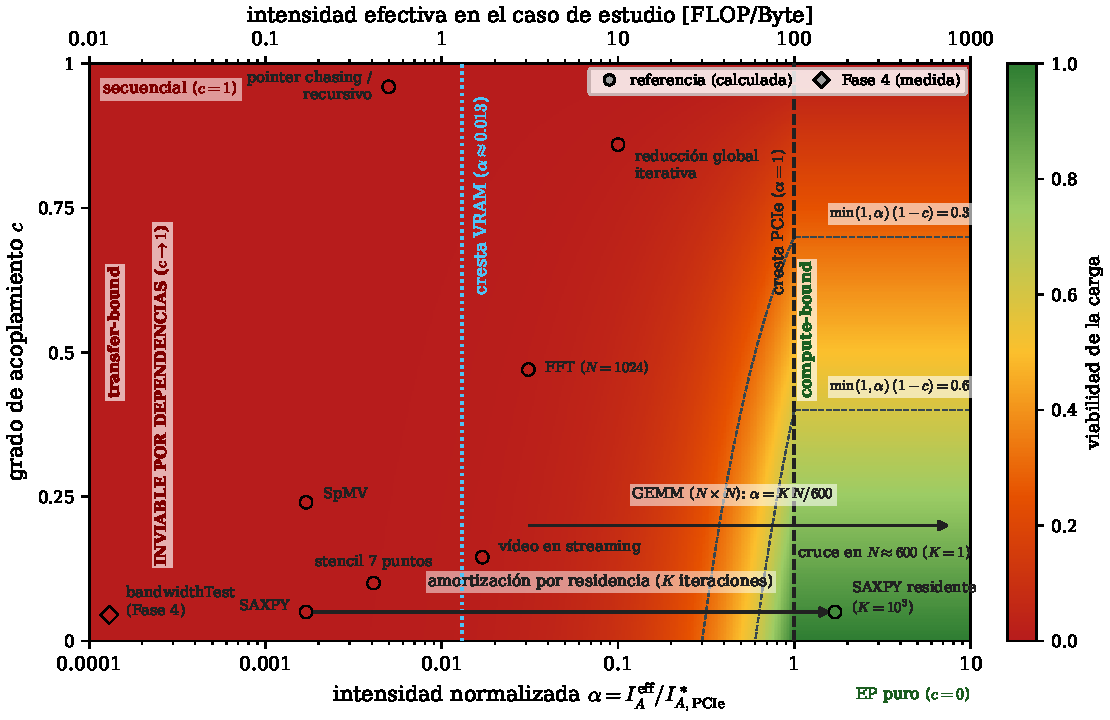
\includegraphics[width=\textwidth]{figuras/mapa_viabilidad.pdf}
    \caption{Mapa de viabilidad de cargas de trabajo, en coordenadas genéricas. El eje horizontal mide la intensidad
    efectiva normalizada por la cresta PCIe, $\alpha = I_{\text{A}}^{\text{eff}} / I_{\text{A,PCIe}}^*$, de modo que la
    frontera \textit{transfer-bound}/\textit{compute-bound} cae siempre en $\alpha = 1$; el eje superior instancia el caso
    de estudio ($\alpha = 1 \leftrightarrow \approx 97$-$103$ FLOP/B). El eje vertical es el grado de acoplamiento $c$
    (\eqref{eq:acoplamiento}) y el color representa $V_{\text{carga}} = F_{\text{carga}}(\alpha) \cdot (1 - c)$, producto
    del filtro de carga por la fracción paralela de Amdahl; las curvas discontinuas oscuras son sus iso-líneas en 0.3 y 0.6,
    y las verticales señalan las crestas PCIe y de VRAM. El rombo es la carga medida en la Fase 4 (\texttt{bandwidthTest}) y
    los círculos, las referencias calculadas con la tabla~\ref{tab:intensidades}. La familia GEMM se representa como una
    trayectoria paramétrica ($\alpha = K\,N/600$), no como un punto, porque su posición depende de $N$ y $K$; cruza la cresta
    en $N \approx 600$ ($K=1$) y diverge al crecer $N$. La flecha muestra la amortización por residencia, que multiplica la
    intensidad efectiva por el número de iteraciones $K$ sobre datos ya presentes en VRAM.}
    \label{fig:mapa}
\end{figure}

\subsection{Procedimiento de clasificación}

La taxonomía se traduce en un procedimiento reproducible para decidir a priori la viabilidad de una carga sobre un sistema
concreto:
\begin{enumerate}[leftmargin=*,itemsep=2pt]
    \item \textbf{Fijar el \textit{working set}} y comprobar si cabe en la VRAM de las tarjetas disponibles (¿es posible la
    residencia?).
    \item \textbf{Estimar $W$ y $B$} por iteración y calcular $I_{\text{A}}^{\text{eff}}$ mediante \eqref{eq:i_eff}.
    \item \textbf{Tomar la ranura más lenta como cota}: comparar $I_{\text{A}}^{\text{eff}}$ con la cresta PCIe de la GPU
    con menor $AB$, que es la que fija el límite del conjunto.
    \item \textbf{Estimar el acoplamiento $c$} mediante perfilado o análisis de dependencias; si $c$ supera el umbral,
    descartar la carga por el eje 2.
    \item \textbf{Evaluar $F_{\text{carga}}$} con \eqref{eq:f_carga} y localizar la carga en la figura~\ref{fig:mapa}.
    \item \textbf{Si cae en zona condicionada}, aplicar transformaciones (bloqueo, residencia, solape de fases, aumento de
    $N$) y repetir el procedimiento; si el techo $I_{\text{A}}^{\max}$ (\eqref{eq:i_max}) no alcanza la cresta, la única vía
    es cambiar de hardware.
\end{enumerate}

\subsection{Ubicación del caso de estudio}

Aplicando el procedimiento anterior a las medidas de la Fase 4:
\begin{itemize}[leftmargin=*,itemsep=2pt]
    \item \texttt{matrixMul} es una carga de familia A/F: EP ($c \approx 0$), con datos residentes durante la ejecución del
    \textit{kernel}, lo que explica que la ejecución concurrente de ambas tarjetas mantuviera el 100\,\% del rendimiento
    individual sin contención apreciable.
    \item \texttt{bandwidthTest} es una carga de familia C: su intensidad efectiva tiende a cero (mueve bytes sin apenas
    cómputo), y por eso su rendimiento coincide con el techo del enlace y no con el de la GPU.
    \item La GTS 250 ocupa la ranura x4 del \textit{chipset} y posee el menor $AB$ ($\approx 0.78$ GB/s); es, por tanto, la
    tarjeta que fija la cota del sistema en el paso 3 del procedimiento. Esta asimetría es la que obliga a repartir la carga
    de forma proporcional a la capacidad de cada GPU ($A_{\text{m}} = \sum_i P_i / P_{\text{ref}}$,
    ecuación~\eqref{eq:am_proporcional}) en lugar de a partes iguales.
\end{itemize}

% ---------------------------------------------------------------------------
\section{Metodología y Resultados Experimentales}

El proyecto ha seguido una metodología secuencial donde cada fase cerró con validación cuantitativa o con el aislamiento riguroso de la causa raíz de inviabilidad:

\subsection*{Fase 1: Aislamiento por Virtualización Completa (VFIO / Máquinas Virtuales)}
\begin{itemize}[leftmargin=*,itemsep=2pt]
    \item \textbf{Objetivo inicial:} Asignar cada tarjeta gráfica a una Máquina Virtual (VM) aislada mediante la tecnología VFIO passthrough. Se optó por este enfoque de cara a la futura incorporación de otras tarjetas, ya que previsiblemente surgirían incompatibilidades de controlador entre ellas.
    \item \textbf{Diagnóstico y Barreras de Hardware:} Durante las pruebas se descubrió que las arquitecturas GT200 y G92b no
    implementan por diseño la capacidad de reinicio por software (son previas a \textit{Function Level Reset}, FLR), exponiendo únicamente métodos de energía (\texttt{reset\_method: pm bus}).
    \item \textbf{Mitigación por Kernel y Fallo en Cascada:} Mediante el ajuste de parámetros de arranque del 
    \textit{kernel} que afectaban a los modos de gestión de energía del bus PCIe (\texttt{pcie\_port\_pm=off}, 
    \texttt{pcie\_aspm=off}, \texttt{vfio\_pci.disable\_idle\_d3=1},
     \texttt{pci=noaer}), se logró sortear el bloqueo inicial de renegociación física del enlace 
     (\textit{link retraining}). No obstante, al intentar inicializar la VM con QEMU/SeaBIOS, la ausencia de soporte 
     para virtualización y la ejecución de resets de bus secundarios forzaron un cuelgue severo en cascada que congeló 
     el bus del anfitrión y provocó tener que montar en modo solo lectura el sistema de archivos (\texttt{ext4 emergency\_ro}).
    \item \textbf{Conclusión Metodológica:} Se documenta que el passthrough por VFIO es inviable y peligroso para la 
    estabilidad del anfitrión en esta generación de GPUs, justificando con evidencia empírica el cambio hacia 
    contenedores de Linux (LXC).
\end{itemize}

\subsection*{Fase 2: Integración del Controlador Legacy en Proxmox VE}
\begin{itemize}[leftmargin=*,itemsep=2pt]
    \item \textbf{Contexto:} Con VFIO, el anfitrión solo asigna las tarjetas al módulo \texttt{vfio-pci} y el controlador se instala dentro de cada máquina virtual, por lo que este paso nunca llegó a abordarse al no arrancar las VMs. Al pasar a contenedores LXC, que comparten el \textit{kernel} del anfitrión, el controlador debe instalarse directamente en Proxmox VE, lo que convierte su integración en el siguiente paso.
    \item \textbf{Objetivo:} Compilar y cargar de forma estable el módulo de kernel NVIDIA 340.108 en un entorno moderno Proxmox VE (Kernel Linux 6.14).
    \item \textbf{Resolución Técnica:} Se superó la brecha de compatibilidad de la API interna del \textit{kernel} aplicando un conjunto de 21 parches mantenidos por la comunidad (\texttt{MichelBoucey/nvidia-340xx}), integrándolos mediante DKMS para asegurar la persistencia ante futuras actualizaciones.
    \item \textbf{Resultado:} El comando \texttt{nvidia-smi} en el anfitrión reconoció de forma inmediata y simultánea 
    las tarjetas conectadas.
\end{itemize}

\subsection*{Fase 3: Linux Containers (LXC) y Puesta a Punto de CUDA 6.5}
\begin{itemize}[leftmargin=*,itemsep=2pt]
    \item \textbf{Objetivo:} Crear un entorno de cómputo aislado que comparta el controlador del anfitrión y permita ejecutar el \textit{runtime} de CUDA 6.5.
    \item \textbf{Resolución técnica:} Se configuró un contenedor LXC privilegiado con paso directo de los
     nodos de dispositivo (\texttt{/dev/nvidia*}) así como se instalaron dentro de él las dependencias relativas a CUDA 
     versión 6.5.
    \item \textbf{Validación de Cómputo Real:} La ejecución de la utilidad oficial \texttt{deviceQuery} completó con éxito (\texttt{Result = PASS}), confirmando que las tarjetas eran capaces de ejecutar código de cálculo paralelo de extremo a extremo.
\end{itemize}

\subsection*{Fase 4: Experimentación, Benchmarks y Medidas de Rendimiento}
\begin{itemize}[leftmargin=*,itemsep=2pt]
    \item \textbf{Superación del Front-End del Compilador:} Para compilar kernels de GPU reales (\texttt{.cu}), el analizador interno de \texttt{nvcc 6.5} (pre-C++11) rechazaba las cabeceras modernas de Debian 12. Se resolvió aislando la compilación dentro de un entorno \textit{chroot} ligero con Debian 8 (Jessie / GCC 4.9.2), generando binarios plenamente funcionales en el contenedor anfitrión.
    \item \textbf{Prueba de Rendimiento de Cómputo (\texttt{matrixMul}):}
    \begin{itemize}[label=$\circ$,itemsep=1pt]
        \item Tesla C1060: \textbf{155.26 GFlop/s}.
        \item GeForce GTS 250: \textbf{80.49 GFlop/s}.
        \item Ratio de rendimiento: $\approx 1.93\times$. Supera la relación de núcleos CUDA ($240/128 \approx 1.88$), y aún más si se tiene en cuenta la mayor frecuencia de \textit{shaders} de la GTS 250, lo que apunta a diferencias de arquitectura entre GT200 y G92b (registros por multiprocesador, ancho de banda de VRAM).
    \end{itemize}
    \item \textbf{Prueba de Ancho de Banda (\texttt{bandwidthTest}):} La transferencia Host$\to$Device alcanzó \textbf{1603.3 MB/s} en la Tesla (slot directo de CPU) frente a \textbf{778.0 MB/s} en la GTS 250 (slot del chipset), arrojando una diferencia de $\mathbf{2.06\times}$. El valor de la GTS 250 se ajusta al techo de una ranura x4 en Gen1 (1 GB/s teórico, $\approx 750$ MB/s efectivos), mientras que el de la Tesla queda por debajo de lo esperable en una ranura x16 ($\approx 3$ GB/s efectivos), por lo que queda pendiente verificar el ancho de enlace negociado.
    \item \textbf{Ejecución Concurrente:} Al ejecutar dos instancias simultáneas de multiplicación matricial pesada, ambas tarjetas mantuvieron el 100\% de su rendimiento individual ($\approx 155.3$ y $\approx 81.3\text{ GFlop/s}$), demostrando que en cargas \textit{compute-bound} no existe penalización ni contención entre dispositivos.
\end{itemize}

% ---------------------------------------------------------------------------
\section{El Marco de Viabilidad Propuesto (\texorpdfstring{$V$}{V})}\label{sec:marcoV}

Para dotar al trabajo de una contribución metodológica aplicable a cualquier otro hardware, se sintetizó el proceso de decisión
mediante un producto de filtros que combina condiciones booleanas y métricas graduadas:
\[
V = \prod_{i} F_i = F_{\text{driver}} \cdot F_{\text{aislamiento}} \cdot F_{\text{carga}} \cdot F_{\text{coste}} \cdot F_{\text{estabilidad}}
\]
La estructura multiplicativa preserva la semántica conjuntiva original: si un solo filtro resulta desfavorable ($F_i = 0$), el
proyecto carece de viabilidad global ($V = 0$). A diferencia de la conjunción booleana, los filtros continuos (como
$F_{\text{carga}}$) ponderan la degradación de forma gradual:

\begin{center}
\small
\begin{tabular}{l>{\raggedright\arraybackslash}p{3.5cm}p{7.5cm}}
\toprule
\textbf{Filtro} & \textbf{Pregunta de Decisión} & \textbf{Diagnóstico en el Caso de Estudio} \\
\midrule
\textbf{F1. Driver} & ¿Compila el controlador en el kernel actual? & \textbf{Favorable:} El controlador 340.108 compila en el kernel 6.14 con 21 parches comunitarios (DKMS). \\
\textbf{F2. Aislamiento} & ¿Requieren las GPUs controladores incompatibles? Si es así, ¿admite el hardware VFIO? & \textbf{Favorable (no aplica):} Pese a pertenecer a arquitecturas distintas (GT200 en las Tesla C1060 y G92b en la GTS 250), 
las tarjetas comparten el controlador 340.108, por lo que basta con LXC. VFIO, previsto para futuras tarjetas con controladores incompatibles, resultó inviable en estas por la ausencia de FLR. \\
\textbf{F3. Carga} & ¿El algoritmo es independiente del bus PCIe? & \textbf{Favorable graduado:} $F_{\text{carga}} = \min(1, I_{\text{A}} \cdot AB / P_{\text{pico}})$, próximo a $1$ en las cargas \textit{compute-bound} medidas (matrices) y decreciente hacia $0$ en transferencias continuas. Desfavorable sin remedio si el techo algorítmico $I_{\text{A}}^{\max}$ no alcanza $I_{\text{A}}^*$. \\
\textbf{F4. Coste} & ¿El beneficio compensa la deuda técnica? & \textbf{Favorable condicionado:} Requiere parches comunitarios activos; sin comunidad el coste de desarrollo lo invalida. \\
\textbf{F5. Estabilidad} & ¿El sistema se mantiene estable en ejecuciones sostenidas? & \textbf{Favorable condicionado:} Con VFIO se produjo un cuelgue en cascada del bus del anfitrión; con LXC la ejecución concurrente se completó sin fallos ni bloqueos. Pendiente de validar en ejecuciones prolongadas. \\
\bottomrule
\end{tabular}
\end{center}

% ---------------------------------------------------------------------------
\section{Modelos de Descomposición y Arquitecturas de Uso}\label{sec:arquitecturas}

La sección~\ref{sec:taxonomia} clasifica \emph{cargas de trabajo}, pero un sistema de cómputo no se despliega por clases de carga, sino
por contratos de uso: la pregunta operativa no es ``¿qué programa es viable?'' sino ``¿qué información debe aportar quien lo ejecuta
para que el sistema pueda aprovecharlo?''. Esta sección da el paso de la carga al despliegue, responde a la pregunta de si la
plataforma podría constituir un \emph{sistema de propósito general} al que cualquier usuario envíe su programa, y precisa qué
arquitecturas de uso quedan disponibles cuando la respuesta es negativa.

% ---------------------------------------------------------------------------
\subsection*{Dos categorías, no un continuo}

Todo modelo de descomposición se sitúa en una de dos categorías, y la frontera entre ambas es de naturaleza informational, no
hardware:

\begin{itemize}[leftmargin=*,labelsep=0.5em,itemsep=0.8ex]
    \item \textbf{Categoría A (automática o transparente):} el usuario entrega un programa secuencial $P$ y el sistema se
    encarga de derivar su descomposición, elegir el modelo y mapear las tareas a los dispositivos. La interfaz es mínima, pero
    exige que el sistema resuelva por sí mismo el problema de la paralelización.
    \item \textbf{Categoría B (declarativa o manual):} el programador aporta la estructura de paralelismo ---la partición, las
    dependencias, el modelo--- como entrada explícita. El sistema se limita a validar, agendar y ejecutar.
\end{itemize}

La primera categoría es la que define a un \emph{sistema de propósito general} de cómputo paralelo, y es precisamente la que
resulta inalcanzable de forma general. La afirmación se apoya en un resultado de indecibilidad, no en una limitación de
implementación:

\begin{quote}\small
\textbf{Teorema (indecidibilidad de la paralelización automática).} No existe un procedimiento efectivo que, dado un programa
secuencial arbitrario $P$ y una máquina objetivo arbitraria, decida si $P$ admite una descomposición paralelo-secuencial
equivalente y con ganancia. En particular, no existe un procedimiento de admisión que clasifique de forma Sound y completa las
cargas que el sistema puede acelerar.
\end{quote}\small

La justificación es directa a partir del \textbf{teorema de Rice}~\cite{rice1953}: la propiedad ``$P$ preserva su semántica bajo una
ejecución particionada y paralelizable'' es una propiedad no trivial de la función que $P$ calcula, y por tanto es indecidible.
En la literatura de \textit{parallel program schemata} el resultado aparece de forma explícita: la conmutabilidad computacional y
propiedades como la terminación o la determinación de un esquema paralelo son indecibles en clases generales
\cite{miller1972}. Las sub-preguntas que la industria se plantea de forma recurrente ---dependencia de valores, dependencia de
memoria y \textit{aliasing} de punteros--- son indecidibles por separado, que es la razón por la que ninguna de las
herramientas de \textit{reverse engineering} de concurrencia es completa.

Lo que sí es decidible son \emph{fragmentos restringidos}. En los programas polihédricos o afines, la resolución de las desigualdades
afines y la partición en bloques se resuelve con aritmética de Presburger, y herramientas como Pluto~\cite{darulova2010} paralelizan
de forma automática y completa esa clase. Pero la pertenencia de un programa arbitrario a ese fragmento vuelve a ser indecidible,
de modo que la paralelización automática solo puede ofrecerse de forma garantizada tras un compromiso explícito del usuario: es exactamente lo
que hacen las \textit{pragmas} de OpenMP, los \textit{scheduling primitives} de Halide o el grafo de flujo de datos que aporta un \textit{framework} como
TensorFlow. Los proyectos de paralelización automática de propósito general hacia GPU de finales de los años 2000
(Stream, Brook, Ocelot) fracasaron precisamente por no cerrar este bucle. La lección de la industria ante un problema indecidible
no fue resolverlo, sino convertir al programador en oráculo: la información que el sistema no puede calcular se exige como
entrada.

Existe un \emph{segundo} impedimento, distinto del anterior y de naturaleza combinatoria. Incluso suponiendo que la
descomposición ya viene dada en la categoría B, decidir qué tarea va a qué GPU de forma óptima es un problema
$P|\text{prec}|C_{\max}$ con aceleradores heterogéneos, que es NP-difícil~\cite{graham1969}. En consecuencia, la expresión
$A_{\text{m}} = \sum_i P_i / P_{\text{ref}}$ de la ecuación~\eqref{eq:am_proporcional} debe leerse como una \textbf{heurística
fundamentada en la medición}, no como un óptimo: reparte en proporción a la capacidad medida porque es la asignación que
iguala los tiempos de finalización, pero no se ha demostrado óptimo para grafos de tareas arbitrarios.

De lo anterior se sigue la respuesta a la pregunta planteada: \textbf{el sistema no puede ser de propósito general}, y la razón
no es que el hardware sea modesto, sino que la generalidad sería una propiedad de la interfaz, no de la máquina. Para ser
precisos, el caso de estudio es de categoría B \emph{por construcción de la cadena de herramientas}: \texttt{nvcc 6.5} nunca ha
incorporado una ruta de paralelización automática de C++, y el paralelismo es siempre explícito en el código fuente
(\texttt{\_\_global\_\_}, \texttt{cudaThreadSynchronize}). La decisión no fue de diseño del proyecto, sino una restricción del
software base disponible, y es coherente con la fase de metodología que muestra el aislamiento ligero por LXC como
sustituto de la virtualización completa.

% ---------------------------------------------------------------------------
\subsection*{Modelos de descomposición del trabajo}

Adoptando como criterio de clasificación \emph{dónde se decide el paralelismo y cuánto tráfico genera entre GPUs}, la literatura
de modelos de programación paralelo~\cite{skillicorn1998,ng2011} puede reducirse a un conjunto acotado de ocho modelos
relevantes para una plataforma de aceleradores con memoria privada. Cada modelo fija el grado de acoplamiento $c$ de
la ecuación~\eqref{eq:acoplamiento} y los bytes que atraviesan el bus, es decir, determina $F_{\text{carga}}$ a través de la
ecuación~\eqref{eq:f_carga}.

\begin{table}[t]
\centering
\footnotesize
\caption{Modelos de descomposición del trabajo, con el coste de acoplamiento $c$ estimado y su diagnóstico sobre la plataforma
del caso de estudio. Los valores de $c$ son estimaciones cualitativas derivadas de la estructura de dependencias de cada
modelo, no medidas directas. La columna de tráfico inter-GPU es el número de travesías de PCIe que el modelo impone por unidad
de trabajo.}
\label{tab:modelos}
\begin{tabular}{>{\raggedright\arraybackslash}p{2.2cm} >{\raggedright\arraybackslash}p{3.9cm} >{\raggedright\arraybackslash}p{2.7cm} >{\raggedright\arraybackslash}p{1.2cm} >{\raggedright\arraybackslash}p{3.7cm}}
\toprule
\textbf{Modelo} & \textbf{Descripción} & \textbf{Tráfico inter-GPU} & \textbf{$c$} & \textbf{Diagnóstico} \\
\midrule
\textbf{M1. Reparto espacial} & Partición del dominio en bloques disjuntos (SIMD/SPMD); cada GPU opera sobre su bloque & $\approx 0$ si el bloque cabe en VRAM & $\approx 0.05$--$0.20$ & \textbf{Viable:} es el medido en la Fase 4 con \texttt{matrixMul} \\
\textbf{M2. Bolsa de tareas} & \textit{Bag-of-tasks} o \textit{master--worker}: unidades independientes encoladas y despachadas sin estructura & $\approx 0$ & $\approx 0.05$ & \textbf{Viable y el más barato:} es el único que no exige conocer la carga \\
\textbf{M3. Robo de trabajo} & Colas locales por hilo; un hilo ocioso roba tareas a un vecino aleatorio (Cilk, TBB) & $\approx 0$ (roboías locales) & $\approx 0.05$--$0.15$ & \textbf{Viable:} cada contenedor LXC es un dominio de robo \\
\textbf{M4. \textit{Fork-join}} & Recursión paralela por divide y vencerás; reducción global al final & $0$ entre hojas & $\approx 0.15$--$0.30$ & \textbf{Viable con precaución:} la reducción final serializa \\
\textbf{M5. Grafo de tareas} & DAG con dependencias explícitas (OmpSs, StarPU, Legion, Taskflow) & 1 por arista que cruza GPU & $\approx 0.20$--$0.40$ & \textbf{Parcial:} solo si las aristas no cruzan dispositivos \\
\textbf{M6. \textit{Pipeline}} & Cadena de etapas que se relevan entre sí (flujo, sistólico) & $2$ por elemento y por frontera & $\approx 0.30$--$0.50$ & \textbf{No:} el relevo se paga en el bus, ecuación~\eqref{eq:hop} \\
\textbf{M7. BSP} & Superpasos separados por barrera global; cómputo local y luego comunicación & $2$ rondas por superpaso & $\approx 0.40$--$0.60$ & \textbf{No:} la barrera global serializa el sistema \\
\textbf{M8. \textit{Dataflow}} & Red de \textit{tokens} activados por dependencias (Kahn, redes de Petri) & según topología de la red & $\approx 0.50$--$0.80$ & \textbf{No:} domina la latencia de los tokens \\
\bottomrule
\end{tabular}
\end{table}

Tres observaciones hacen de la tabla~\ref{tab:modelos} un instrumento de decisión y no un simple catálogo. La primera es que
M5 \emph{generaliza} a M6 y M7: un \textit{pipeline} es un camino en el grafo de tareas y un superpaso BSP es un grafo completo
por capas, de modo que la elección útil para un implementador se reduce en realidad a cinco modelos (M1--M5). La segunda es
que el diagnóstico de M6--M8 no se debe a su intensidad aritmética ---una etapa densa de un \textit{pipeline} sería
perfectamente \emph{compute-bound}---, sino a su $c$ alto: mueren por el término $(1-c)$ de la cota de Amdahl, no por el bus. La
tercera es que la causa estructural es común a M5--M8 y merece nombrarse aparte.

\subsection*{Por qué el relevo entre GPUs es irrompible}

Las tarjetas de este trabajo (GT200 y G92b, anteriores a la aparición del acceso entre pares sobre PCIe) no implementan
comunicación directa entre dispositivos. Todo relevo entre dos GPUs debe por tanto descargar en la memoria del anfitrión y
volver a subir, lo que convierte una frontera de una etapa en \textbf{dos} travesías del bus. El coste por unidad de trabajo es:
\begin{equation}\label{eq:hop}
    T_{\text{relé}} = \frac{2b}{AB \cdot \eta \cdot \gamma}
\end{equation}
donde $b$ son los bytes del intermedio, y $\eta$ y $\gamma$ son la eficiencia de protocolo y el factor de contención de la
sección~\ref{sec:topologia}. El factor $2$ es la diferencia entre un buen diseño y uno inviable, y es lo que separa M5 de M6--M8
en la tabla~\ref{tab:modelos}.

El relevo solo se amortiza si cada etapa realiza suficiente cómputo sobre el intermedio. Igualando el tiempo de cómputo de la
etapa con el de su relevo, y sustituyendo $W = I_{\text{A}} b$ y $P_{\text{pico}}$, resulta el umbral:
\begin{equation}\label{eq:hop_umbral}
    I_{\text{A}} > \frac{2\,P_{\text{pico}}}{AB \cdot \eta} = \frac{2}{\eta}\,I_{\text{A}}^*
\end{equation}
Es decir, con $\eta \approx 0.75$ un \textit{pipeline} entre GPUs exige más del \emph{doble} de la intensidad aritmética del punto
de cresta, y no solo superarlo, para no quedar limitado por el propio relevo. Con los valores medidos en la Fase 4, ese umbral
se sitúa en $\approx 258$ FLOP/B en la Tesla C1060 y $\approx 276$ FLOP/B en la GTS 250, muy por encima de las
$\approx 97$--$103$ FLOP/B de la sección~\ref{sec:roofline}. Ninguna de las cargas de la tabla~\ref{tab:intensidades} alcanza
ese umbral en su forma \textit{streaming}; solo el producto denso de matrices lo supera, y para superarlo necesita residencia en
VRAM, precisamente la condición que un \textit{pipeline} entre tarjetas no puede ofrecer.

% ---------------------------------------------------------------------------
\subsection*{La ventana de trabajo del sistema}

El reparto espacial M1 introduce un criterio de dimensionamiento que no aparece en las secciones anteriores: la capacidad total
de VRAM del sistema. Con 4 GB en cada Tesla C1060 y 1 GB en la GTS 250, el sistema solo aporta una ventaja sobre una GPU
suelta cuando el \emph{working set} supera la VRAM de la tarjeta más grande y no supera la suma de todas:
\begin{equation}\label{eq:ventana}
    \underbrace{\max_i \text{VRAM}_i}_{4\ \text{GB}} < W \le \underbrace{\sum_i \text{VRAM}_i}_{9\ \text{GB}}
\end{equation}
La cota inferior es inmediata: por debajo de 4 GB el problema se resuelve íntegramente en una sola tarjeta. La cota superior
es la relevante: por encima de 9 GB el \emph{working set} ya no cabe en el conjunto y la carga se convierte en \emph{out-of-core},
es decir, familia C de la tabla~\ref{tab:familias}, con $\alpha \to 0$ y $F_{\text{carga}} \to 0$.

Dentro de esa ventana el reparto espacial no genera tráfico inter-GPU, de modo que el bus solo se ve afectado por la transferencia
de entrada, y la carga queda en la familia A o F. Cuantitativamente, para un producto denso de matrices de precisión simple, el
conjunto $A$, $B$ y $C$ ocupa $12N^2$ bytes, luego:
\begin{itemize}[leftmargin=*,itemsep=2pt]
    \item $W = 4$ GB corresponde a $N \approx 18\,300$, y $W = 9$ GB a $N \approx 27\,400$.
    \item En todo ese rango la intensidad aritmética vale $I_{\text{A}} = N/6 \approx 3\,050$--$4\,560$ FLOP/B, entre $30\times$ y
    $46\times$ el punto de cresta, por lo que $F_{\text{carga}} = 1$ de forma robusta y no marginal.
    \item El tiempo de cómputo en el extremo inferior de la ventana es del orden de $\approx 31$ s usando la capacidad agregada
    medida ($2 \times 155.26 + 80.49 = 391$ GFlop/s), lo que sitúa la ventana en el rango de trabajos por lotes (\emph{batch})
    donde el tiempo de puesta en marcha puede amortizarse y $F_{\text{coste}}$ deja de penalizar.
\end{itemize}
La ventana~\eqref{eq:ventana} es, por tanto, un resultado de dimensionamiento que se sigue directamente de las medidas y que
no habría sido deducible del análisis teórico: define el rango de problemas para el que reunir estas tarjetas concretas aporta
algo que no aporta una sola de ellas.

% ---------------------------------------------------------------------------
\subsection*{Arquitecturas de uso viables}

Si el sistema no puede ser de propósito general, la pregunta relevante es qué arquitecturas de uso sobreviven y bajo qué
condición. La tabla~\ref{tab:arquitecturas} las recoge, con los filtros del marco~\ref{sec:marcoV} dominantes en cada una y el
punto de fallo explícito.

\begin{table}[t]
\centering
\footnotesize
\caption{Arquitecturas de uso del sistema, con el compromiso de información que cada una impone, los filtros dominantes y su
punto de fallo. Todas ellas pertenecen a la categoría B, con la excepción parcial de M2/M3, que solo exigen al usuario declarar la
independencia de las tareas y no su estructura interna.}
\label{tab:arquitecturas}
\begin{tabular}{>{\raggedright\arraybackslash}p{2.8cm} >{\raggedright\arraybackslash}p{2.6cm} >{\raggedright\arraybackslash}p{3.4cm} >{\raggedright\arraybackslash}p{5.4cm}}
\toprule
\textbf{Arquitectura} & \textbf{Modelo} & \textbf{Filtros dominantes} & \textbf{Condición de validez y punto de fallo} \\
\midrule
\textbf{Acelerador especializado de un tenant} & M1, M2 & $F_{\text{carga}}$, $F_{\text{coste}}$ & Válida para familias A, B y F con $c$ bajo. Falla si aparece una carga de familia D (\emph{sincronización fina}), donde la cota de Amdahl es independiente del número de GPUs \\
\textbf{Distribuidor de trabajos independientes} & M2, M3 & $F_{\text{carga}}$, $F_{\text{estabilidad}}$ & Solo exige al cliente declarar independencia entre unidades de trabajo, no su estructura. Es la interfaz más próxima a un servicio general, y aun así no puede aceptar una carga no caracterizada: la clasificación de la tabla~\ref{tab:familias} sigue siendo responsabilidad del cliente \\
\textbf{\textit{Pipeline} por fases particionadas} & M5, M6 & $F_{\text{carga}}$ & Solo viable si cada etapa es familia A y el relevo se amortiza, es decir $I_{\text{A}} > (2/\eta)\,I_{\text{A}}^*$ (ecuación~\eqref{eq:hop_umbral}). Falla en cuanto aparece una frontera entre GPUs con intermedio grande \\
\textbf{Coprocessor PCIe desagregado} & M1 & $F_{\text{carga}}$, $F_{\text{coste}}$ & El anfitrión conserva el código secuencial y delega solo el \emph{kernel} denso. Falla por latencia de ida y vuelta si el \emph{kernel} delegado es pequeño: en Gen1 la ida y vuelta domina el cómputo \\
\textbf{Nodo oportunista en un clúster heterogéneo} & M2 & $F_{\text{coste}}$ & Se usa en huecos o en tareas de prioridad baja, aprovechando el bajo coste marginal de la energía en horas valle frente a una máquina moderna equivalente. Falla en latencia: no puede competir con un servicio Xeon en tiempo de respuesta \\
\textbf{Banco de pruebas del propio marco} & M1 & $F_{\text{driver}}$, $F_{\text{aislamiento}}$, $F_{\text{estabilidad}}$ & Uso meta: valida el marco de viabilidad de la sección~\ref{sec:marcoV} sobre hardware nuevo sin exigirle rendimiento. No es un uso de producción y no está sujeto a $F_{\text{coste}}$ \\
\bottomrule
\end{tabular}
\end{table}

% ---------------------------------------------------------------------------
\subsection*{Corolario: el compromiso es parte de la arquitectura}

Las dos categorías se reducen ahora a una consecuencia operativa. Como no existe procedimiento de admisión que decida si una
carga arbitraria es paralelizable con ganancia, un sistema que pretenda ser de propósito general solo puede operar
en modo \emph{best effort}: admitir la carga y descubrir en ejecución que no se paraleliza, lo que es exactamente la
combinación de $f_{\text{m}}$ desconocido y $S \le 1/(1-f_{\text{m}})$ de la ecuación~\eqref{eq:amdahl_limite}. Frente a esa
incertidumbre, la estrategia de la arquitectura es \emph{fijar el compromiso por adelantado}: cada arquitectura de la
tabla~\ref{tab:arquitecturas} declara qué información exige del programador, qué familias de carga acepta y qué techo
sostiene. No es un sistema que descubra el paralelismo, sino uno que lo exige.

El marco de viabilidad propuesto en la sección~\ref{sec:marcoV} cierra el argumento. Para que un sistema fuera de propósito general tendría que
servir todas las familias de la tabla~\ref{tab:familias}, y por la estructura multiplicativa de $V$ su valor quedaría fijado por
la peor de ellas:
\begin{equation}\label{eq:v_general}
    V_{\text{general}} = \min_{\text{familias}} V
    \;\le\; F_{\text{carga}}\big|_{\text{familia C}}
    \;\approx\; 0.0017 \;\approx\; 0
\end{equation}
con independencia de que $F_{\text{driver}}$, $F_{\text{aislamiento}}$, $F_{\text{coste}}$ y $F_{\text{estabilidad}}$ resulten
favorables. Esto es, la no-generalidad de la plataforma no es un defecto corregible con mejor hardware ni con más tarjetas: es
una propiedad estructural de la semántica del paralelismo, y se manifiesta en el marco exactamente donde la taxonomía de las
cargas choca con la del hardware. La consecuencia práctica es que el valor del trabajo no está en haber construido un
acelerador heterogéneo rentable, sino en haber establecido los límites dentro de los cuales ese acelerador tiene sentido, y en
que esos límites son calculables antes de invertir esfuerzo.

% ---------------------------------------------------------------------------
\section{Posicionamiento Frente a la Tecnología Actual}\label{sec:posicionamiento}

Las secciones anteriores evalúan un único sistema. Esta sección aplica el mismo marco a la generación actual de hardware,
con dos objetivos que conviene separar: determinar \emph{dónde está hoy} esta plataforma frente a las alternativas disponibles en
el mercado, y comprobar si el marco de la sección~\ref{sec:marcoV} es transferible o si está moldeado por el caso de estudio.

Se establece de entrada una distinción de evidencia, en la línea de la introducida en la tabla~\ref{tab:intensidades}: los valores
de $P_{\text{pico}}$ y $AB$ del sistema objeto de este trabajo son \textbf{medidos} en la Fase 4, mientras que los de las
plataformas de referencia son \textbf{especificaciones de fabricante}~\cite{nvidiac1060,nvidiartxblackwell,nvidiaproblackwell,nvidiablackwellultra,nvidiahgx} y
no han sido verificados experimentalmente en este trabajo. La conclusión que se derive de ellos es, por tanto, una estimación
soportada, no una medida. Tampoco se emplean precios de compra, por no ser un dato reproducible: el mercado de segunda mano de
tarjetas de esta generación no tiene precio de referencia estable, y fijarlo debilitaría más la conclusión de lo que la
sostendría.

\subsection*{Plataformas de referencia}

La tabla~\ref{tab:comparativa} recoge las plataformas de referencia. Se incluyen seis, que cubren el salto desde el consumo
actual hasta el segmento profesional y de centro de datos, más el propio anfitrión del caso de estudio, que es una referencia
relevante porque ya está en la máquina y porque su rendimiento no depende de ninguna tarjeta.

\begin{table}[t]
\centering
\footnotesize
\setlength{\tabcolsep}{3.5pt}
\caption{Plataformas de referencia frente al sistema objeto de este trabajo. $P_{\text{pico}}$ es potencia de cálculo FP32
vectorial; $AB$ es el ancho de banda de memoria local, e $I_{\text{A}}^{*} = P_{\text{pico}}/AB$ el punto de cresta resultante,
que es la magnitud que determina si un \textit{kernel} resident es \emph{compute-bound} o no. Las cifras de las plataformas de
referencia son especificaciones de fabricante~\cite{nvidiac1060,nvidiartxblackwell,nvidiaproblackwell,nvidiablackwellultra,nvidiahgx};
las del sistema propio son medidas en la Fase 4, y su $AB$ y su TDP son la suma de los valores de ficha de las tres tarjetas.
Para el anfitrión, $P_{\text{pico}}$ es el pico teórico y su valor real en HPL es de 1\,011 GFLOP/s~\cite{puget7950x}. El
descenso de $I_{\text{A}}^{*}$ en las dos últimas filas no indica una mejora arquitectónica, sino la magnitud del ancho de banda
HBM: son productos cuyo pico FP32 es irrelevante frente a su capacidad tensorial.}
\label{tab:comparativa}
\begin{tabular}{>{\raggedright\arraybackslash}p{3.6cm} c c c c c c c}
\toprule
\textbf{Plataforma} & \textbf{Año} & \textbf{$P_{\text{pico}}$} & \textbf{$AB$} & \textbf{$I_{\text{A}}^{*}$} & \textbf{VRAM} & \textbf{TDP} & \textbf{GFLOP/W} \\
& & \textbf{[GFLOP/s]} & \textbf{[GB/s]} & \textbf{[FLOP/B]} & & \textbf{[W]} & \\
\midrule
\textbf{Sistema propio (3 GPUs, agregado)} & 2009 & \textbf{391} & 166 & \textbf{2,4} & 9 GB & 338 & 1,2 \\
\textbf{Anfitrión sin acelerador (7950X)} & 2022 & 2\,920 & 83 & -- & -- & 170 & 17,2 \\
\textbf{Consumo media-alta (RTX 5070 Ti 16 GB)} & 2025 & 43\,940 & 896 & 49\,000 & 16 GB & 300 & 146 \\
\textbf{Consumo alta (RTX 5090 32 GB)} & 2025 & 104\,800 & 1\,792 & 58\,500 & 32 GB & 575 & 182 \\
\textbf{Workstation (RTX PRO 6000 Blackwell)} & 2025 & 126\,000 & 1\,792 & 70\,300 & 96 GB & 600 & 210 \\
\textbf{Centro de datos actual (B300 SXM)} & 2025 & 75\,000 & 8\,000 & 9\,375 & 288 GB & 1\,400 & 53,6 \\
\textbf{Centro de datos entrante (Rubin SXM)} & 2026 & 130\,000 & 22\,000 & 5\,900 & 288 GB & n.d. & -- \\
\bottomrule
\end{tabular}
\end{table}

Las cifras de la tabla~\ref{tab:comparativa} permiten un solo tipo de afirmación defendible: la de orden de magnitud. Los ratios
que se derivan a continuación son relaciones entre un dato medido y un dato de ficha técnica, y deben leerse como tales.

Dos advertencias sobre la lectura de la tabla evitan conclusiones erróneas. La primera es que el B300, pese a ser la cúspide de
la generación, \textbf{no es un producto de cómputo de propósito general}: su cómputo FP64 es de 1,25 TFLOPS por GPU frente a
los 37 TFLOPS del B200, una reducción del 97\,\% que NVIDIA compensa con 14 PFLOP/s de FP4~\cite{nvidiablackwellultra}. Para
cargas de doble precisión, la comparación pertinente es con un H100, un H200 o el Rubin entrante, no con el B300. La segunda es
que el descenso de $I_{\text{A}}^{*}$ en las dos últimas filas no representa una mejora de eficiencia: es el efecto de la HBM, y
significa que esas plataformas son aún más difíciles de saturar en FP32 vectorial que una tarjeta de consumo.

\subsection*{El sistema no es competitivo en términos absolutos}

El dato más incómodo para la hipótesis inicial del trabajo es que \textbf{la CPU que ya reside en la plataforma lo supera}. Una
publicación de evaluación del Ryzen 9 7950X con compiladores optimizados para Zen 4 reporta 1\,011 GFLOP/s en el \textit{benchmark}
estándar HPL~\cite{puget7950x}. Esa cifra es 2,6 veces la capacidad agregada medida de las tres GPUs del sistema (391 GFLOP/s), y
ese cómputo se realiza con software que no depende de ninguna tarjeta, sin compilaciones exóticas y con un controlador con soporte
oficial. En potencia de pico FP32 la diferencia es de 7,5 veces a favor del procesador.

El segundo ratio es el energético. Las tres tarjetas suman 338 W de potencia de diseño y entregan 391 GFLOP/s, es decir, 1,2
GFLOP/W, mientras que una tarjeta de consumo actual entrega 146 GFLOP/W y una estación profesional, 210 GFLOP/W. La eficiencia
del sistema reutilizado es, por tanto, entre 122 y 175 veces peor según el término de comparación. Aplicando la ecuación del
modelo económico de la sección~\ref{sec:economia}, con la energía como único coste cuantificable de forma
reproducible, el filtro $F_{\text{coste}}$ del sistema propio es \emph{desfavorable}, y lo es por un margen de dos órdenes de
magnitud que ningún ajuste de software puede corregir.

La conclusión que se impone es directa y no admite matiz: \textbf{si el objetivo es obtener cómputo al menor precio, la opción
válida es comprar una tarjeta actual}, incluso una de gama media, y el sistema aquí estudiado no es una alternativa a ella. La
sección~\ref{sec:economia} se deja abierta precisamente porque el coste de adquisición del hardware heredado, no medido aquí,
es el único término que podría desplazar el resultado, y su signo es conocido: el mercado de segunda mano de tarjetas GT200 y
G92b tiene precio próximo a cero, lo que hace el sistema propio más barato en adquisición pero no en funcionamiento, y dado que
la diferencia en cómputo va de 112 a 332 veces según la plataforma, el ahorro de adquisición no compensa el coste energético en el
horizonte de vida útil de la plataforma.

\subsection*{El punto de cresta: el único rasgo favorable}

Existe sin embargo un resultado derivado del marco que sí favorece al hardware antiguo, y que merece enunciarse con precisión
porque es contraintuitivo. La cuarta columna de la tabla~\ref{tab:comparativa} muestra que el punto de cresta de memoria del
sistema propio es de 2,4 FLOP/B, mientras que el de las plataformas de referencia es entre 3\,900 y 29\,000 veces mayor: la
tarjeta de hace más de una década alcanza su techo de cómputo con una intensidad aritmética tres o cuatro órdenes de magnitud
inferior. La razón es que el diseño de las GPUs actuales ha desplazado la inversión desde los vectores FP32 hacia los núcleos
tensoriales, de modo que su techo vectorial es tan alto que ningún \textit{kernel} de FP32 convencional lo alcanza: una tarjeta
de consumo actual es, en la práctica, \emph{VRAM-bound} para casi toda carga densa, y solo se acerca a su techo mediante
teselado agresivo o con TF32. Las dos filas de centro de datos reducen esa distancia a un factor de 3\,900--4\,100, y no por
eficiencia vectorial sino porque su ancho de banda HBM es enorme; conviene no confundir ambos efectos.

Esto explica, y no justifica, el resultado de la Fase 4. Las tres tarjetas heredadas mantuvieron el 100\,\% de su rendimiento
individual en ejecución concurrente porque, con un punto de cresta de 2,4 FLOP/B, el producto denso de matrices se sitúa muy por
encima de su techo y no hay nada que optimizar. Es una propiedad de robustez en la utilización, no de potencia: la tarjeta antigua
es mucho más fácil de saturar y mucho más lenta. Un \textit{kernel} de GEMM bien escrito alcanza quizá el 60\,\% del techo de una
tarjeta de consumo actual y el 100\,\% del de la C1060, y sigue siendo decenas de veces más rápido en la tarjeta moderna.

\subsection*{La ventana de capacidad deja de ser un diferencial}

La ventana~\eqref{eq:ventana} de la sección~\ref{sec:arquitecturas} se había construido como la única ventaja estructural del
sistema: ofrece una capacidad de VRAM superior a la de una tarjeta individual, con 9 GB frente a los 4 GB de la C1060. Esa
ventana deja de ser un diferencial en cuanto se comparan las plataformas de referencia, que ofrecen 16, 32, 96 y 288 GB en una
sola tarjeta. Cualquier carga que quepa en la suma de las VRAM del sistema propietario cabe holgadamente en una tarjeta actual, y
con un techo de cómputo entre 112 y 332 veces superior. La ventana no es un nicho: está estrictamente contenida en el dominio de
una tarjeta moderna, y su único efecto es el contrario del buscado, porque la carga que la aprovecha es la que peor
aprovechamiento ofrece en la plataforma antigua respecto a su propio techo.

\subsection*{Qué es realmente lo que se paga en un sistema profesional}

El argumento de mercado para el hardware profesional no es el rendimiento, y el caso de estudio ofrece una razón concreta para
afirmarlo. En la Fase 1, el aislamiento por passthrough VFIO fue inviable y provocó un cuelgue en cascada del bus del anfitrión
que dejó el sistema de archivos en modo de solo lectura. Ese fallo no es un accidente ni una mala configuración: es la
consecuencia directa de que las arquitecturas GT200 y G92b son anteriores al \textit{Function Level Reset} del PCIe 2.1 y no
admiten reinicio por software, de modo que el sistema no puede devolver un dispositivo fallido a un estado conocido. El
componente de precio de un equipo profesional existe para comprar la ausencia de ese problema, no para comprar FLOPs.

Las plataformas de referencia ofertan precisamente los mecanismos que el caso de estudio no pudo obtener. La generación actual de
centro de datos incorpora \textbf{MIG}, particionado en hasta siete instancias con memoria, caché y núcleos de cómputo aislados
\emph{a nivel de hardware}~\cite{nvidiablackwellultra}: es exactamente el aislamiento que el VFIO debía proporcionar y que la
generación de este hardware no permite obtener por software. En el segmento profesional se añaden la corrección de errores en
memoria, el soporte de \textit{virtual GPU} con perfiles dedicados y, hasta la generación Ampere, un enlace NVLink de 112,5 GB/s
entre dos tarjetas~\cite{nvidiaa6000}; ese enlace ha desaparecido del segmento de workstation en las generaciones posteriores, de
modo que hoy el fabric entre tarjetas es exclusivo del centro de datos. En cualquier caso, los 112,5 GB/s de las dos últimas
tarjetas con NVLink superan en un factor de 70 a las dos travesías del bus Gen1 que cualitativamente la ecuación~\eqref{eq:hop}
impone a cualquier relevo entre las tarjetas de este trabajo. La diferencia entre ambas generaciones, resumida, es que la
profesional vende garantía de aislamiento y la heredada no puede ofrecerla a ningún precio.

\subsection*{Presupuesto de carriles PCIe: cuántas GPUs caben}

La pregunta de cuántas tarjetas admite la plataforma tiene una respuesta contable. El Ryzen 9 7950X expone 28 carriles PCIe 5.0,
repartidos en el bloque de 16 carriles que alimenta la ranura principal, dos grupos de 4 para almacenamiento y el enlace de 4
carriles hacia el \textit{chipset}. Con el enlace forzado a Gen1, cada carril rinde 250 MB/s efectivos una vez descontada la
codificación 8b/10b, de modo que x4 equivale a 1 GB/s teórico y x16 a 4 GB/s.

Esa aritmética permite además reinterpretar las medidas de la Fase 4, y lo hace de forma que conviene señalar porque cierra uno de
los puntos que la metodología dejó abiertos. La transferencia de \textbf{1603,3 MB/s} de la Tesla no corresponde a un enlace x16,
que daría del orden de 3,2 GB/s al 80\,\% de eficiencia, sino a un enlace \textbf{x8}, cuyo valor teórico es 2 GB/s y cuya
eficiencia resultante es del 80,2\,\%. La GTS 250, con 778,0 MB/s sobre un x4 teórico de 1 GB/s, ofrece una eficiencia del
77,8\,\%. Las tres tarjetas presentan por tanto la misma eficiencia de enlace, y la lectura más parsimoniosa es que la ranura
principal está bifurcada en x8/x8 para las dos Tesla y que ninguna de ellas dispone de 16 carriles. Procede confirmarlo leyendo
directamente el ancho negociado (\texttt{LnkCap}/\texttt{LnkSta}) en lugar de inferirlo, porque el ajuste entre las dos cifras y
un rendimiento del 80\,\% es exacto al 0,2\,\%.

El presupuesto ideal de carriles, tomando los 4 carriles por tarjeta como ancho mínimo viable, es entonces:
\begin{itemize}[leftmargin=*,itemsep=2pt]
    \item 16 carriles de CPU, bifurcados en x4/x4/x4/x4: \textbf{4 GPUs}.
    \item 4 carriles del enlace de \textit{chipset}: \textbf{1 GPU} más, compartida con discos, red y USB.
\end{itemize}
\textbf{Total: 5 GPUs en el caso ideal}, frente a las 3 que el sistema aloja realmente. Conviene retener una propiedad que es el eje
de todo lo que sigue: \emph{la bifurcación y los conmutadores PCIe multiplican el número de ranuras, nunca el ancho de banda}. Si
se necesitan más tarjetas de las que permiten los carriles de CPU, la única vía es un conmutador PCIe, que reparte el mismo enlace
de subida entre todas ellas.

\subsection*{Cuántas GPUs aportan cómputo y cuántas no}

La composición del Roofline con el reparto espacial decide cuánto aporta cada tarjeta sin necesidad de más supuestos. Como el cupo
de datos de cada GPU es independiente y el rendimiento agregado es la suma, el rendimiento útil del conjunto es la suma de los
rendimientos individuales, cada uno limitado por su propio enlace:
\begin{equation}\label{eq:util}
    P_{\text{útil}}(I_A) = \sum_i \min\left(P_i,\; I_A \cdot AB_i\right)
\end{equation}
La lectura de \eqref{eq:util} es por tarjeta: cuando $I_A$ supera $P_i / AB_i$, la GPU está en su techo de cómputo y aporta todo lo
que puede; por debajo, aporta exactamente los FLOPs que su enlace permite alimentar. \textbf{Añadir una tarjeta solo añade cómputo
si el enlace de esa tarjeta lo permite}, esto es, si $I_A > P_i / AB_i$. Con los valores medidos, ese umbral por tarjeta es de
$\approx 97$ FLOP/B en las Tesla (sobre x8) y $\approx 103$ FLOP/B en la GTS 250, que son los valores que ya aparecían en el mapa
de viabilidad. Pero si el objetivo es escalar hasta el presupuesto ideal de 5 carriles, cada tarjeta quedaría a x4, con 750 MB/s
efectivos, y el umbral se elevaría a $\approx 207$ FLOP/B: el paso de x8 a x4 se paga duplicando la intensidad exigida.

La comparación entre la configuración real y la ideal cuantifica la ganancia de escalar:
\begin{itemize}[leftmargin=*,itemsep=2pt]
    \item \textbf{Configuración real} (3 GPUs: dos a x8 y una a x4): 3,99 GB/s agregados, 391 GFLOP/s de techo, cresta de
    $\approx 98$ FLOP/B.
    \item \textbf{Configuración ideal} (5 GPUs a x4): 3,75 GB/s agregados, 776 GFLOP/s de techo, cresta de $\approx 207$ FLOP/B.
\end{itemize}
El resultado es abrupto y merece subrayarse: \textbf{la configuración que maximiza el número de GPUs tiene un 6\,\% menos de ancho
de banda agregado que la configuración real}, porque bifurcar el x16 en cuatro carriles entrega menos ancho por tarjeta del que
entregaba la ranura x8. La escalera de ampliación no es monótona: por debajo de $I_A \approx 105$ FLOP/B la configuración de 3
GPUs iguala o supera a la de 5, hasta un 6\,\% mejor, porque ambas quedan limitadas por su enlace agregado; en $I_A \approx 105$
FLOP/B hay empate; y solo por encima de ese valor la configuración de 5 domina, acercándose a $2\times$ en el límite.

Dicho de otro modo: \textbf{el cruce entre ambas arquitecturas cae exactamente sobre el punto de cresta del sistema actual}. Por
debajo de él, escalar el número de tarjetas no aporta nada, y solo es útil para cargas de alta intensidad, donde el techo de
cómputo crece mientras el bus permanece constante en unos 4 GB/s. El caso extremo lo ilustra el carril x1, estándar en los
\textit{risers} de minería: 250 MB/s elevarían el umbral a $\approx 621$ FLOP/B, por encima de todas las cargas de la
tabla~\ref{tab:intensidades} salvo el producto denso de matrices en su régimen asintótico.

\subsection*{Mantenibilidad y disponibilidad frente al número de tarjetas}

El escalado por acumulación tiene un segundo coste que no es de ancho de banda, y que la Fase 1 deja a la vista. En el
mantenimiento del software base el coste es constante en el número de tarjetas: las tres comparten el controlador 340.108 y los
21 parches comunitarios, de modo que pasar de tres a cinco no añade trabajo de integración. Es la única dimensión en la que
escalar esta plataforma sale gratis.

La disponibilidad, en cambio, se degrada de forma superlineal. Ninguna de las arquitecturas implicadas admite \textit{Function
Level Reset}, así que el fallo o el intento de reinicio de una sola tarjeta no se contiene en esa tarjeta: se propaga al bus del
anfitrión, y la Fase 1 documenta exactamente ese resultado, con el bus congelado y el sistema de archivos en modo de solo lectura.
La disponibilidad del conjunto no es la del promedio de las tarjetas, sino la de la peor de ellas, y con $N$ tarjetas la
probabilidad de que alguna provoque un evento crece con $N$ mientras el coste de cada evento es el 100\,\% del sistema. En una
plataforma con FLR y MIG, el mismo evento degrada la capacidad en una fracción de $1/N$ y el servicio continúa. La diferencia
entre ambos modelos es, por tanto, \textbf{cuadrática en el número de tarjetas}: el coste esperado de indisponibilidad crece como
$N^2$ en la plataforma heredada y permanece constante en la profesional. Escalar por acumulación es, en esta generación, escalar
el riesgo.

\subsection*{Cómo escalan las alternativas}

La comparación se cierra con el modo en que cada alternativa resuelve el problema de crecer, que es donde el contraste de enfoque
resulta más nítido: en horizontal (\emph{scale-out}), acumulando dispositivos, o en vertical (\emph{scale-up}), sustituyéndolos
por uno mayor.

\begin{table}[t]
\centering
\footnotesize
\setlength{\tabcolsep}{4pt}
\caption{Mecanismos de escalado de las alternativas. La columna de ancho de banda por GPU es la magnitud decisiva: es la que fija
el punto de cresta de cada plataforma y, con él, el conjunto de cargas que puede saturar. Los valores de las plataformas de
referencia son especificaciones de fabricante.}
\label{tab:escalado}
\begin{tabular}{>{\raggedright\arraybackslash}p{2.8cm} >{\raggedright\arraybackslash}p{2.3cm} >{\raggedright\arraybackslash}p{1.7cm} >{\raggedright\arraybackslash}p{2.2cm} >{\raggedright\arraybackslash}p{1.9cm} >{\raggedright\arraybackslash}p{3.0cm}}
\toprule
\textbf{Plataforma} & \textbf{Mecanismo} & \textbf{GPUs alcanzables} & \textbf{PCIe a host} & \textbf{Fabric entre GPUs} & \textbf{Coste de mantenimiento} \\
\midrule
\textbf{Este sistema} (2009) & Escalado horizontal (\emph{scale-out}): acumular tarjetas repartiendo carriles & 5 (carriles); 3 al nivel real & \textbf{1,6 GB/s} (Gen1 x8, medido) & \textbf{Ninguno} & 21 parches comunitarios, sin FLR, fallo total en cascada \\
\textbf{Consumo actual} (2025) & Escalado vertical (\emph{scale-up}), no horizontal & 1--2 & 63 GB/s (Gen5 x16) & Ninguno & Controlador oficial hasta el fin de vida del modelo \\
\textbf{Workstation} (2025) & Escalado vertical (\emph{scale-up}) & 1--2 & 63 GB/s (Gen5 x16) & No ofrecido & ECC, homologación y ciclo de vida \\
\textbf{Centro de datos actual} (B300) & NVSwitch 5 & 8 (HGX) -- 72 (NVL72) & 128 GB/s (Gen6 x16) & 900 GB/s & MIG, ECC, telemetría, sustitución en caliente \\
\textbf{Centro de datos entrante} (Rubin) & NVLink 6 & 8 -- 576 & 128 GB/s (Gen6 x16) & 1\,800 GB/s & ídem \\
\textbf{Nube} & Elástico, bajo demanda & Sin límite práctico & La del proveedor & La del proveedor & Ninguno: se externaliza \\
\bottomrule
\end{tabular}
\end{table}

Las dos columnas de ancho de banda de la tabla~\ref{tab:escalado} están deliberadamente separadas porque son canales distintos y
no deben compararse entre sí. El primero es el enlace con el anfitrión, que es el que alimenta el \emph{working set} desde la
memoria del sistema; el segundo es la red entre tarjetas, que solo transporta intermedios una vez los datos residen ya en VRAM.
Es la distinción que la ecuación~\eqref{eq:hop} convierte en coste, y en la plataforma heredada el segundo canal simplemente no
existe: \emph{no hay fabric}, de modo que todo relevo entre tarjetas paga dos travesías del primero. Todas las cifras se expresan
en un sentido para que sean comparables con la medición de \texttt{bandwidthTest} de la Fase 4; las fichas técnicas publican
habitualmente el valor bidireccional, que es el doble.

El contraste de la tabla~\ref{tab:escalado} resume la conclusión: \textbf{la plataforma heredada es la única de las alternativas
cuyo mecanismo de escalado no aumenta el ancho de banda}, y cada generación posterior multiplica el enlace por 39 (consumo) o 80
(centro de datos) veces, reservando el fabric para el segmento profesional y de centro de datos. El crecimiento por acumulación
solo compensa mientras cada tarjeta conserve sus propios carriles, lo que agota el presupuesto físico en el tercer o cuarto
dispositivo; a partir de ahí el escalado exige compartir, y el umbral de intensidad exigido se eleva con cada tarjeta añadida. En
el resto de alternativas la restricción no está en el número de dispositivos sino en el precio, y ese es el motivo por el que la
estrategia del mercado es el escalado vertical (\emph{scale-up}), con una sola tarjeta grande, y no el horizontal
(\emph{scale-out}).

\subsection*{Lo que sí sobrevive: patrimonio de software}

Queda un nicho en el que la conclusión se invierte, y es el único defendible sin matices. Un binario compilado con CUDA 6.5 para
las arquitecturas \texttt{sm\_11} y \texttt{sm\_13} que definen estas tarjetas \emph{no puede ejecutarse en ninguna GPU
actual}, y no puede recompilarse, porque el compilador que lo produjo y la API de la que depende ya no existen para las
generaciones posteriores. En ese caso el coste de la plataforma heredada no es alternativo al de una tarjeta moderna, sino el
único modo de ejecución posible, y la comparación de la tabla~\ref{tab:comparativa} deja de ser pertinente. Este es el escenario
de patrimonio software y de controladores industriales heredados, y es el único en el que la palabra \emph{viabilidad} conserva
su sentido pleno.

A este argumento se añade un segundo, ya Implícito en el anterior: cuando el hardware ya está en el aula o en el laboratorio y su
coste marginal de adquisición es cero, la comparación de la tabla~\ref{tab:comparativa} no es el término relevante, porque no hay
decisión de compra que tomar. El sistema entonces no compite con el mercado, y su justificación es formativa y experimental, que es
precisamente el objetivo del presente trabajo.

\subsection*{Transferibilidad del marco}

La aplicación del marco de la sección~\ref{sec:marcoV} a las plataformas de la tabla~\ref{tab:comparativa} produce la
tabla~\ref{tab:filtros}, y su resultado más relevante no es el veredicto de cada fila, sino que \textbf{los cinco filtros no se
comportan de forma homogénea frente al hardware}. Dos de ellos, $F_{\text{driver}}$ y $F_{\text{aislamiento}}$, son enteramente
dependientes de la generación: favorables en el hardware actual, desfavorables en el heredado. $F_{\text{carga}}$ es favorable en
todos los casos y no discrimina entre ellos, lo que confirma que su valor es un techo y no un veredicto. $F_{\text{coste}}$ es
desfavorable tanto en el sistema propio como en el profesional, pero por razones opuestas: en el primero por eficiencia, en el
segundo por precio de adquisición, y solo se vuelve favorable en el modelo de pago por uso, donde una A100 de 40 GB ---ya dos
generaciones por detrás del B300--- se alquila entre 0,67 y 3,67 \$ por GPU y hora~\cite{cloudgpus}, de modo que el alquiler elimina
la barrera de adquisición pero no la de eficiencia. $F_{\text{estabilidad}}$ es el único filtro cuya dirección se invierte por
generación, y lo hace de forma tajante: desfavorable en el heredado, que carece de soporte, de ciclo de vida y de reinicio por
software, y favorable en el profesional y el centro de datos.

\begin{table}[t]
\centering
\footnotesize
\caption{Comportamiento de los cinco filtros del marco frente a la generación del hardware. La disparidad entre filas es el
resultado relevante: un marco útil debe producir diagnósticos distintos según la plataforma, no un veredicto único.}
\label{tab:filtros}
\begin{tabular}{>{\raggedright\arraybackslash}p{2.6cm} >{\raggedright\arraybackslash}p{3.4cm} >{\raggedright\arraybackslash}p{3.4cm} >{\raggedright\arraybackslash}p{3.4cm}}
\toprule
\textbf{Filtro} & \textbf{Hardware heredado} & \textbf{Consumo actual} & \textbf{Profesional / centro de datos} \\
\midrule
$F_{\text{driver}}$ & Desfavorable: 21 parches comunitarios, sin soporte oficial & Favorable: controlador con ciclo de vida activo & Favorable \\
$F_{\text{aislamiento}}$ & No aplicable: LXC compartido, sin FLR & No aplicable o vGPU parcial & Favorable: MIG con aislamiento hardware \\
$F_{\text{carga}}$ & Graduado: favorable solo en la ventana~\eqref{eq:ventana} & Favorable en todo el mapa de viabilidad & Favorable \\
$F_{\text{coste}}$ & Desfavorable: 1,2 GFLOP/W & Favorable & Desfavorable en compra, favorable en pago por uso \\
$F_{\text{estabilidad}}$ & Desfavorable: sin ciclo de vida, cuelgue de bus en VFIO & Favorable & Favorable: ECC, aislamiento, redundancia \\
\bottomrule
\end{tabular}
\end{table}

De este contraste se sigue la validación del método. Un marco de decisión que solo sabe decir ``no'' no es contrastable, y uno que
solo sabe decir ``sí'' tampoco. El marco propuesto es contrastable en ambas direcciones: aplicado al caso de estudio pronostica
favorable el cómputo denso y desfavorable la carga de transferencia, que es exactamente lo que midió la Fase 4, y aplicado a las
plataformas de referencia habría pronosticado $F_{\text{coste}} \approx 0$ desde el primer día, antes de construir nada. La
contribución del trabajo no es, por tanto, el sistema construido, sino un procedimiento que predice su propio caso de estudio y
que se niega a sí mismo cuando el hardware no lo merece.

\subsection*{El enlace como variable del marco}

El coste de relevo de la ecuación~\eqref{eq:hop} no es una propiedad de estas tarjetas, sino de cualquier frontera entre dos
dispositivos. Generalizado al número $h$ de travesías del enlace que la cruza, y con la eficiencia de protocolo $\eta$ de
\eqref{eq:hop_umbral}:
\begin{equation}\label{eq:frontera}
    T_{\text{frontera}} = \frac{h\,b}{AB \cdot \eta},
    \qquad\text{y el umbral asociado}\qquad
    I_{\text{A}}^{\text{min}} = \frac{h\,P_{\text{pico}}}{AB \cdot \eta}
\end{equation}
El caso $h=1$ corresponde al acceso directo entre dispositivos (P2P o NVLink) y $h=2$ al relevo a través de la memoria del
anfitrión, que es el de la ecuación~\eqref{eq:hop}. Con esta lectura el marco se aplica sin cambios a topologías que no dependen
de un mismo anfitrión ---una GPU por nodo unida por red, un clúster de placas SBC con GPU externa, varias GPU bajo un mismo
\textit{root complex}---, basta sustituir $AB$ y $h$. La tabla~\ref{tab:enlaces} particulariza el umbral para los enlaces
representativos de esas topologías.

\begin{table}[t]
\centering
\footnotesize
\setlength{\tabcolsep}{5pt}
\caption{Umbral de intensidad por frontera para distintos enlaces, calculado con~\eqref{eq:frontera} y $\eta = 0,75$. Todas las
filas usan la RTX 5070 Ti de la tabla~\ref{tab:comparativa} ($P_{\text{pico}} = 43\,940$ GFLOP/s) salvo la del sistema propio,
que usa su $P_{\text{pico}}$ medido; el umbral escala linealmente con $P_{\text{pico}}$, de modo que una tarjeta mayor lo eleva
en la misma proporción. Los anchos de los enlaces de referencia son especificaciones de fabricante; los del sistema propio son
medidos. Son estimaciones calculadas, no medidas, y valen como tales.}
\label{tab:enlaces}
\begin{tabular}{>{\raggedright\arraybackslash}p{4.0cm} c c c >{\raggedright\arraybackslash}p{5.2cm}}
\toprule
\textbf{Enlace} & \textbf{$AB$ [GB/s]} & \textbf{$h$} & \textbf{$I_{\text{A}}^{\text{min}}$} & \textbf{Diagnóstico} \\
\midrule
Ethernet 10 GbE & 1,25 & 2 & $\approx 93\,700$ & Solo M2/M3: sin fronteras que amortizar \\
RoCE 200 GbE directo~\cite{nvidiadgxspark} & 25 & 2 & $\approx 4\,700$ & M2/M3 y réplicas; M6 en el extremo denso de la ventana~\eqref{eq:ventana} \\
PCIe Gen5 x4 sin P2P (GeForce) & 15,75 & 2 & $\approx 7\,400$ & M2/M4 y réplicas; M6 solo asintótico; TP y FSDP penalizados \\
PCIe Gen5 x16 con P2P (profesional) & 63 & 1 & $\approx 930$ & M6 y TP con holgura \\
NVLink profesional (A6000)~\cite{nvidiaa6000} & 112,5 & 1 & $\approx 520$ & M5--M8 viables \\
\midrule
\textbf{Este sistema} (Gen1 x8, C1060) & \textbf{1,6} & \textbf{2} & $\approx 258$ & M1--M4; solo el GEMM residente supera el umbral \\
\bottomrule
\end{tabular}
\end{table}

Tres lecturas se siguen de la tabla. La primera es que el problema del sistema propio no es de época, sino de umbral: las GPU de
consumo actuales carecen de fabric entre tarjetas (tabla~\ref{tab:escalado}), de modo que el relevo vuelve a pagar $h=2$, ahora
sobre Gen5 x4; con un $P_{\text{pico}}$ 283 veces mayor y una travesía diez veces más ancha, el umbral resultante es casi treinta
veces más exigente que el medido aquí. Lo que cambia respecto a 2009 no es la estructura del coste, sino su escala. La segunda es
que la red no elimina la frontera, la desplaza: a 10 GbE ninguna carga de la tabla~\ref{tab:intensidades} alcanza el umbral, y a
200 GbE solo las densas residentes se acercan; en cambio, para M2/M3 cualquier enlace sirve, porque no hay fronteras que cruzar.
La tercera es que la sincronización por capa (TP, FSDP) no se rige por~\eqref{eq:frontera} sino por la latencia de cada colectiva,
y sin P2P cada una paga las dos travesías del anfitrión más la latencia del \textit{root complex}: el mismo mecanismo que la
tabla~\ref{tab:escalado} describe para este sistema. Un nodo SBC con GPU externa añade, además, su propia travesía de Gen3 x1
antes de la red, de modo que no mejora ninguna fila. El marco no está, por tanto, moldeado por el caso de estudio: aplicado a
cualquier topología falla o absuelve por la misma razón ---el umbral de intensidad frente al punto de cresta del enlace--- y solo
NVLink, hoy exclusivo del centro de datos, compra el $h=1$ que las cargas acopladas necesitan.

\begin{thebibliography}{99}

\bibitem{amdahl1967}
E.~M. Amdahl.
\newblock \emph{Validity of the single processor approach for achieving large scale computing capabilities}.
\newblock \emph{AFIPS Spring Joint Computer Conference}, pp.~483--485, 1967.

\bibitem{gustafson1988}
J.~L. Gustafson.
\newblock \emph{The limits of parallelism: Amdahl's law in general purpose multicomputers}.
\newblock \emph{Communications of the ACM}, 31(8), pp.~474--479, 1988.

\bibitem{williams2009}
S.~Williams, A.~Waterman y D.~Patterson.
\newblock \emph{Roofline: an insightful visual performance model for multicore architectures}.
\newblock \emph{Communications of the ACM}, 52(4), pp.~65--76, 2009.

\bibitem{flynn1972}
M.~J. Flynn.
\newblock \emph{Some computer organizations with extensible parallelism}.
\newblock \emph{IEEE Transactions on Computers}, C-21(9), pp.~948--958, 1972.

\bibitem{rice1953}
H.~G. Rice.
\newblock \emph{Classes of subclasses and computability}.
\newblock \emph{Transactions of the American Mathematical Society}, 74, pp.~358--366, 1953.

\bibitem{miller1972}
R.~E. Miller.
\newblock \emph{Some undecidability results for parallel program schemata}.
\newblock \emph{Conference on Proving Assertions about Programs}, IBM Research, 1972.

\bibitem{graham1969}
R.~L. Graham, D.~L. Knuth y S.~M. Patil.
\newblock \emph{Optimal scheduling for two-processor systems}.
\newblock \emph{AFIPS Spring Joint Computer Conference}, pp.~225--232, 1969.

\bibitem{valiant1990}
L.~G. Valiant.
\newblock \emph{A model of parallel computation in polymorphic parallel systems}.
\newblock \emph{Journal of the ACM}, 37(3), pp.~483--493, 1990.

\bibitem{culler1993}
D.~E. Culler, R.~M. Karp, D.~Patterson, A.~Sahay, K.~E. Schauser, E.~M. Santos,
R.~E. Subramonian y T.~von Sickel.
\newblock \emph{LogP: towards a realistic model of parallel computation}.
\newblock \emph{ACM SIGPLAN Symposium on Principles and Practice of Parallel Programming (PPoPP)}, pp.~1--12, 1993.

\bibitem{frigo1998}
M.~Frigo, D.~Foster y S.~Ghuloum.
\newblock \emph{Strand-aware multithreading in Cilk}.
\newblock \emph{IEEE International Parallel and Distributed Processing Symposium (IPDPS)}, pp.~136--146, 1998.

\bibitem{skillicorn1998}
D.~B. Skillicorn.
\newblock \emph{Models and languages for parallel computation}.
\newblock \emph{ACM Computing Surveys}, 30(2), pp.~123--169, 1998.

\bibitem{ng2011}
C.~K.~H. Ng, D.~Holmes y S.~Green.
\newblock \emph{Parallel programming models: a comparison and assessment}.
\newblock \emph{International Journal of Parallel Programming}, 39(5), pp.~449--480, 2011.

\bibitem{gillies2018}
C.~Gillies, J.~Pearce, C.~Malliaris y S.~Pop.
\newblock \emph{A taxonomy of task-based parallel programming technologies for high-performance computing}.
\newblock \emph{The Journal of Supercomputing}, 74(3), 2018.

\bibitem{darulova2010}
L.~Darulova y A.~Rothvoß.
\newblock \emph{Pluto: a polyhedral automatic parallelization tool for C/C++}.
\newblock \emph{ACM/IEEE International Conference on Computer-Aided Design (ICCAD)}, pp.~506--515, 2010.

\bibitem{kung1980}
H.~T. Kung y C.~E. Leiserson.
\newblock \emph{Systolic algorithms}.
\newblock \emph{IEEE Transactions on Computers}, C-29(3), pp.~297--308, 1980.

\bibitem{nvidiac1060}
NVIDIA.
\newblock \emph{Tesla C1060 computing processor board: product specification}.
\newblock \emph{Product Brief}, NVIDIA Corporation, 2010.
\newblock \url{https://www.nvidia.com/docs/IO/56483/BD-04111-001_v05.pdf}.

\bibitem{nvidiartxblackwell}
NVIDIA.
\newblock \emph{NVIDIA RTX Blackwell GPU architecture}.
\newblock \emph{Technical Whitepaper}, NVIDIA Corporation, 2025.
\newblock \url{https://images.nvidia.com/aem-dam/Solutions/geforce/blackwell/nvidia-rtx-blackwell-gpu-architecture.pdf}.

\bibitem{nvidiaproblackwell}
NVIDIA.
\newblock \emph{NVIDIA RTX PRO Blackwell GPU architecture}.
\newblock \emph{Technical Whitepaper}, NVIDIA Corporation, 2025.
\newblock \url{https://www.nvidia.com/content/dam/en-zz/Solutions/design-visualization/quadro-product-literature/NVIDIA-RTX-Blackwell-PRO-GPU-Architecture-v1.0.pdf}.

\bibitem{nvidiablackwellultra}
NVIDIA.
\newblock \emph{NVIDIA Blackwell Ultra: datasheet}.
\newblock NVIDIA Corporation, 2025.
\newblock \url{https://resources.nvidia.com/en-us-blackwell-architecture/blackwell-ultra-datasheet/}.

\bibitem{nvidiahgx}
NVIDIA.
\newblock \emph{NVIDIA HGX platform: system specifications}.
\newblock NVIDIA Corporation, 2026.
\newblock \url{https://www.nvidia.com/en-us/data-center/hgx/}.

\bibitem{nvidiaa6000}
NVIDIA.
\newblock \emph{NVIDIA RTX A6000: datasheet}.
\newblock NVIDIA Corporation, 2020.
\newblock \url{https://www.nvidia.com/content/dam/en-zz/Solutions/Data-Center/a6000/pdf/nvidia-rtx-a6000-datasheet.pdf}.

\bibitem{nvidiadgxspark}
NVIDIA.
\newblock \emph{DGX Spark user guide: ConnectX-7 networking}.
\newblock NVIDIA Corporation, 2026.
\newblock \url{https://docs.nvidia.com/dgx/dgx-spark/spark-clustering.html}.

\bibitem{puget7950x}
Puget Systems.
\newblock \emph{Zen 4 AVX-512 performance with AMD AOCCv4: HPL, HPCG and HPL-MxP results}.
\newblock \emph{Technical Analysis}, 2023.
\newblock \url{https://www.pugetsystems.com/labs/hpc/ryzen-7950x-zen4-avx512-performance-with-amd-aoccv4-hpl-hpcg-hpl-mxp/}.

\bibitem{cloudgpus}
Cloud GPUs.
\newblock \emph{NVIDIA A100 40GB SXM: cloud rental price comparison across 8 providers}.
\newblock \url{https://cloud-gpus.com/nvidia-a100-40gb-sxm/}.

\bibitem{michelboucey}
M.~Boucey.
\newblock \emph{nvidia-340xx DKMS driver: parches de compatibilidad para \textit{kernels} contemporáneos}.
\newblock \url{https://github.com/MichelBoucey/nvidia-340xx}.

\end{thebibliography}

\end{document}
